%!TEX root = ../main.tex
\chapter{Proceso de desarrollo de la Ontología}
\label{chap:Desarrollo de la Ontologia}

Luego de haber estudiado las distintas metodologías para el desarrollo de ontologías se decidió utilizar la metodología NeOn ya que la misma, según lo que se muestra en la Tabla  \ref{tab:comparacion} de la seccion \ref{chap:Marco Teorico}, posee mayor especificación en las actividades a desarrollar  y contempla los casos de reuso de recursos ontológicos y no-ontológicos. 

Siguiendo la metodología NeOn, se identifica que la ontología a desarrollar sigue las actividades compuestas principalmente por los escenarios 1, 2 y 3 que se exponen en la metodología. El escenario 1, puesto que se quiere modelar una ontología desde el principio y es la base de los demás escenarios, el escenario 2 y 3 ya que se pretende reusar recursos ontológicos y no-ontológicos respectivamente. Los desarrollos ontológicos pueden pertenecer a uno o mas escenarios, los escenarios elegidos sirven como guía para el desarrollo de la ontología. A continuación se detalla la primera actividad de la metodología, que consiste en la especificación de los requerimiento de la ontología.


\section{Especificación de requerimientos de la ontología}

En esta actividad se define el alcance y los requerimientos de la ontología a desarrollar. Como resultado de esta actividad se obtiene el Documento de Especificación de Requerimientos de la Ontología (ORSD). A continuación se detalla el resultado de dicho proceso.
\begin{enumerate}

    \begin{figure}[h!]
        \centering
        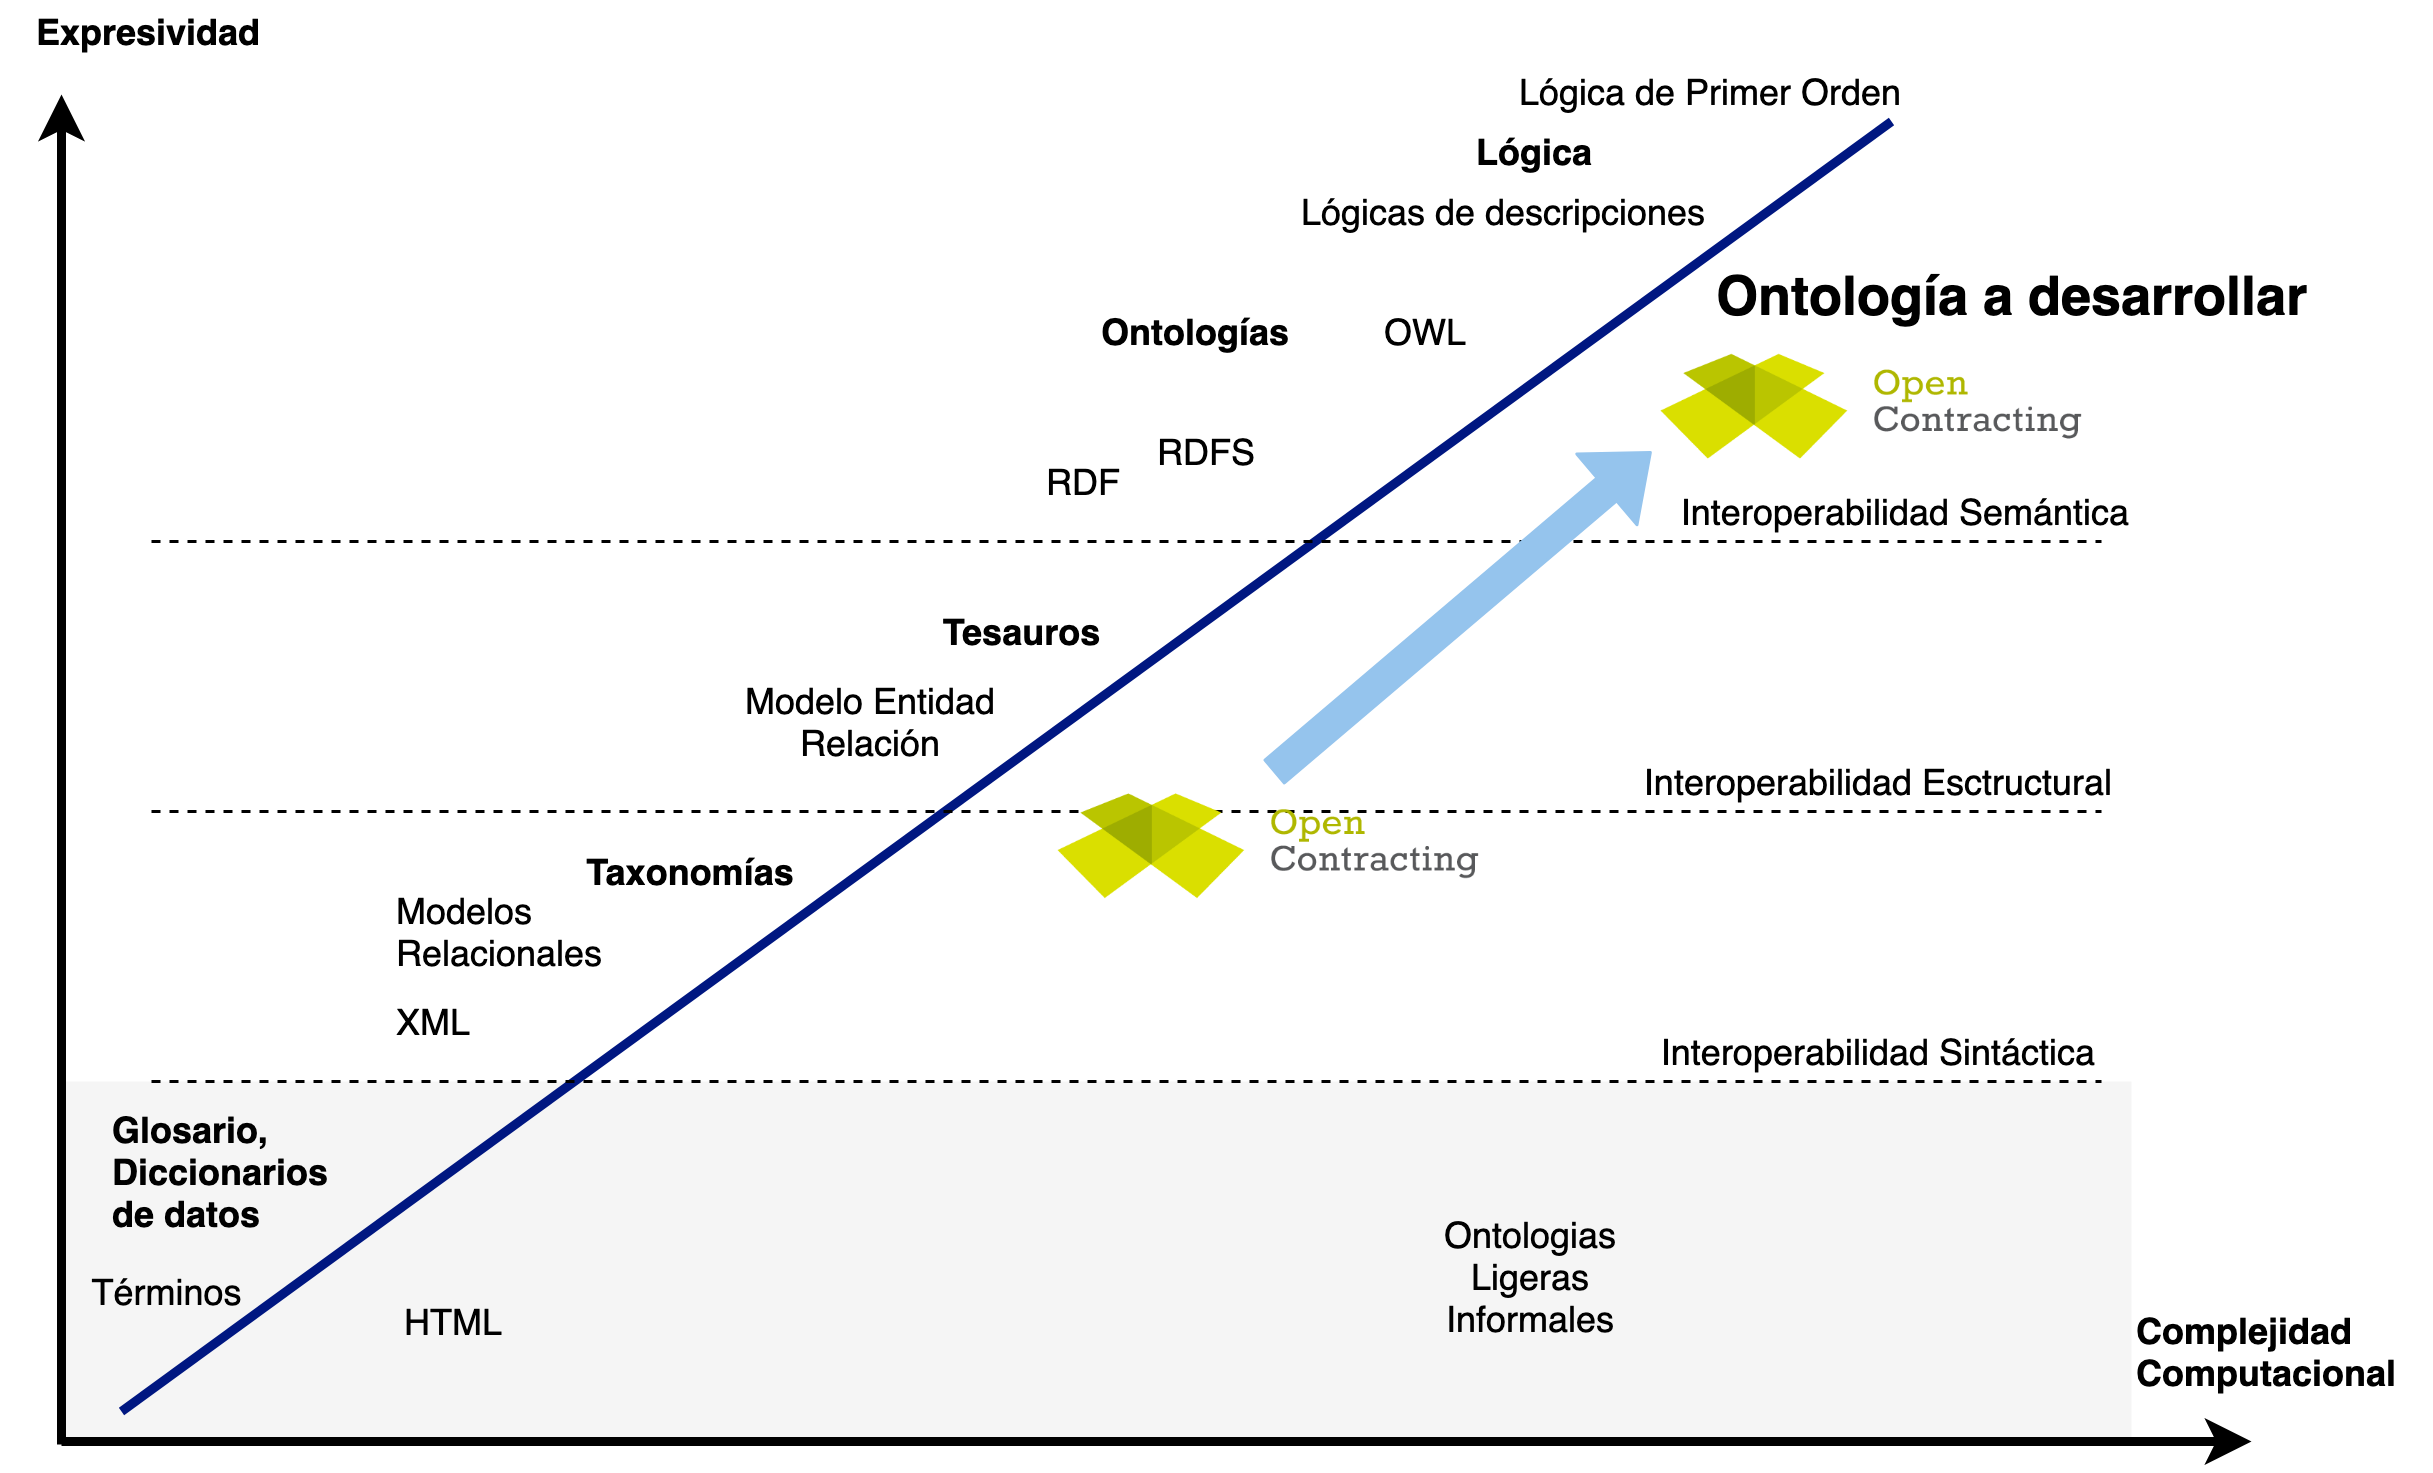
\includegraphics[width=150mm]{figuras/Diagramas-OenContracting.png}
        \caption{Nivel de complejidad semantica de la ontologia a desarrollar}
        \label{img:ocds-ocntology-complejidad}
        \end{figure}
        
\item \textbf{Propósito:} Crear una ontología para el dominio de Contrataciones Públicas para lograr la interoperabilidad semántica con otras fuentes de datos externas utilizando el OCDS como base de conocimiento principal aumentando la formalidad semántica como se muestra en la figura \ref{img:ocds-ocntology-complejidad}


\item \textbf{Alcance:} El alcance de la ontología está delimitada por el vocabulario detallado en la versión 1 del OCDS. Se eligió dicha versión ya en el momento del inicio de esta investigación era la última versión estable del estándar.
\item \textbf{Lenguaje de Implementación.} Se utilizará el lenguaje OWL debido a que es el lenguaje preferido para ontologías en la web semántica recomendado por la W3C \cite{OWLSeman72:online}, y se requiere de una ontología lo suficientemente ligera y explícita que se pueda manejar en la web semántica.
\item \textbf{Grupo Objetivo.}La ontología está orientada a:
\begin{enumerate}
    \item Expertos del dominio de Contrataciones Públicas que quieran realizar consultas ad-hoc sobre datos.
    \item Desarrolladores de software que deseen implementar el OCDS.
    \item Desarrolladores de software que necesiten integrar datos de contrataciones públicas con otras fuentes externas. \end{enumerate}
\item \textbf{Usos de la Ontología. }La ontología se utilizará para crear un esquema de publicación en JSON-LD, esto es debido a que la sintaxis JSON es ampliamente conocida y preferida por los desarrolladores \cite{JSON-37:online}, además el OCDS ya posee un esquema de publicación compatible con esta sintaxis. Los datos utilizados se extraerán del portal de datos abiertos de la DNCP.
\item \textbf{Requerimientos No Funcionales: }
\begin{enumerate}
    \item Se optará, en lo posible, por la reutilización de otras ontologías del dominio de Contrataciones Públicas ampliamente utilizadas.
    \item La ontología desarrollada debe ser procesable dentro de las limitaciones de la web semántica, ósea debe ser una ontología ligera.
    \item Debe soportar múltiples lenguajes: inglés y español inicialmente.
\end{enumerate}
\item \textbf{Requerimientos Funcionales. }
    \begin{enumerate}
        \item Gracias a la ontología se podrán responder las mismas preguntas que se responden a través de los datos publicados en formato de JSON y se podrán responder preguntas de todas las fases del proceso licitatorio.
        \item Debe ser compatible con la versión 1 del OCDS.
        \item Los datos deberán poder ser enriquecidos con otras fuentes de datos provenientes de la DNCP y también fuentes externas como Wikidata o DBpedia.
    \end{enumerate}
\item \textbf{Pre-Glosario de Términos.} El glosario fue extraído del diccionario de datos y de la ontología desarrollada por la DNCP. 
\end{enumerate}


\section{Planificación de las actividades}

Aquí se define el modelo de ciclo de vida de la ontología. El ciclo de vida que se adapta a los escenarios elegidos es el Modelo de Cascada de 6 fases, debido a que serán necesarias las fases de reuso tanto de recursos ontológicos como no-ontológicos, reingeniería, y diseño para la implementación. En la Figura \ref{img:secuenciaDeDesarrollo} se muestra el modelo de ciclo de vida a seguir. Se decidió utilizar el Modelo de Ciclo de Vida Cascada ya que el alcance de la ontología es bien delimitado y el tiempo acotado.

\begin{figure}[ht!]
    \centering
    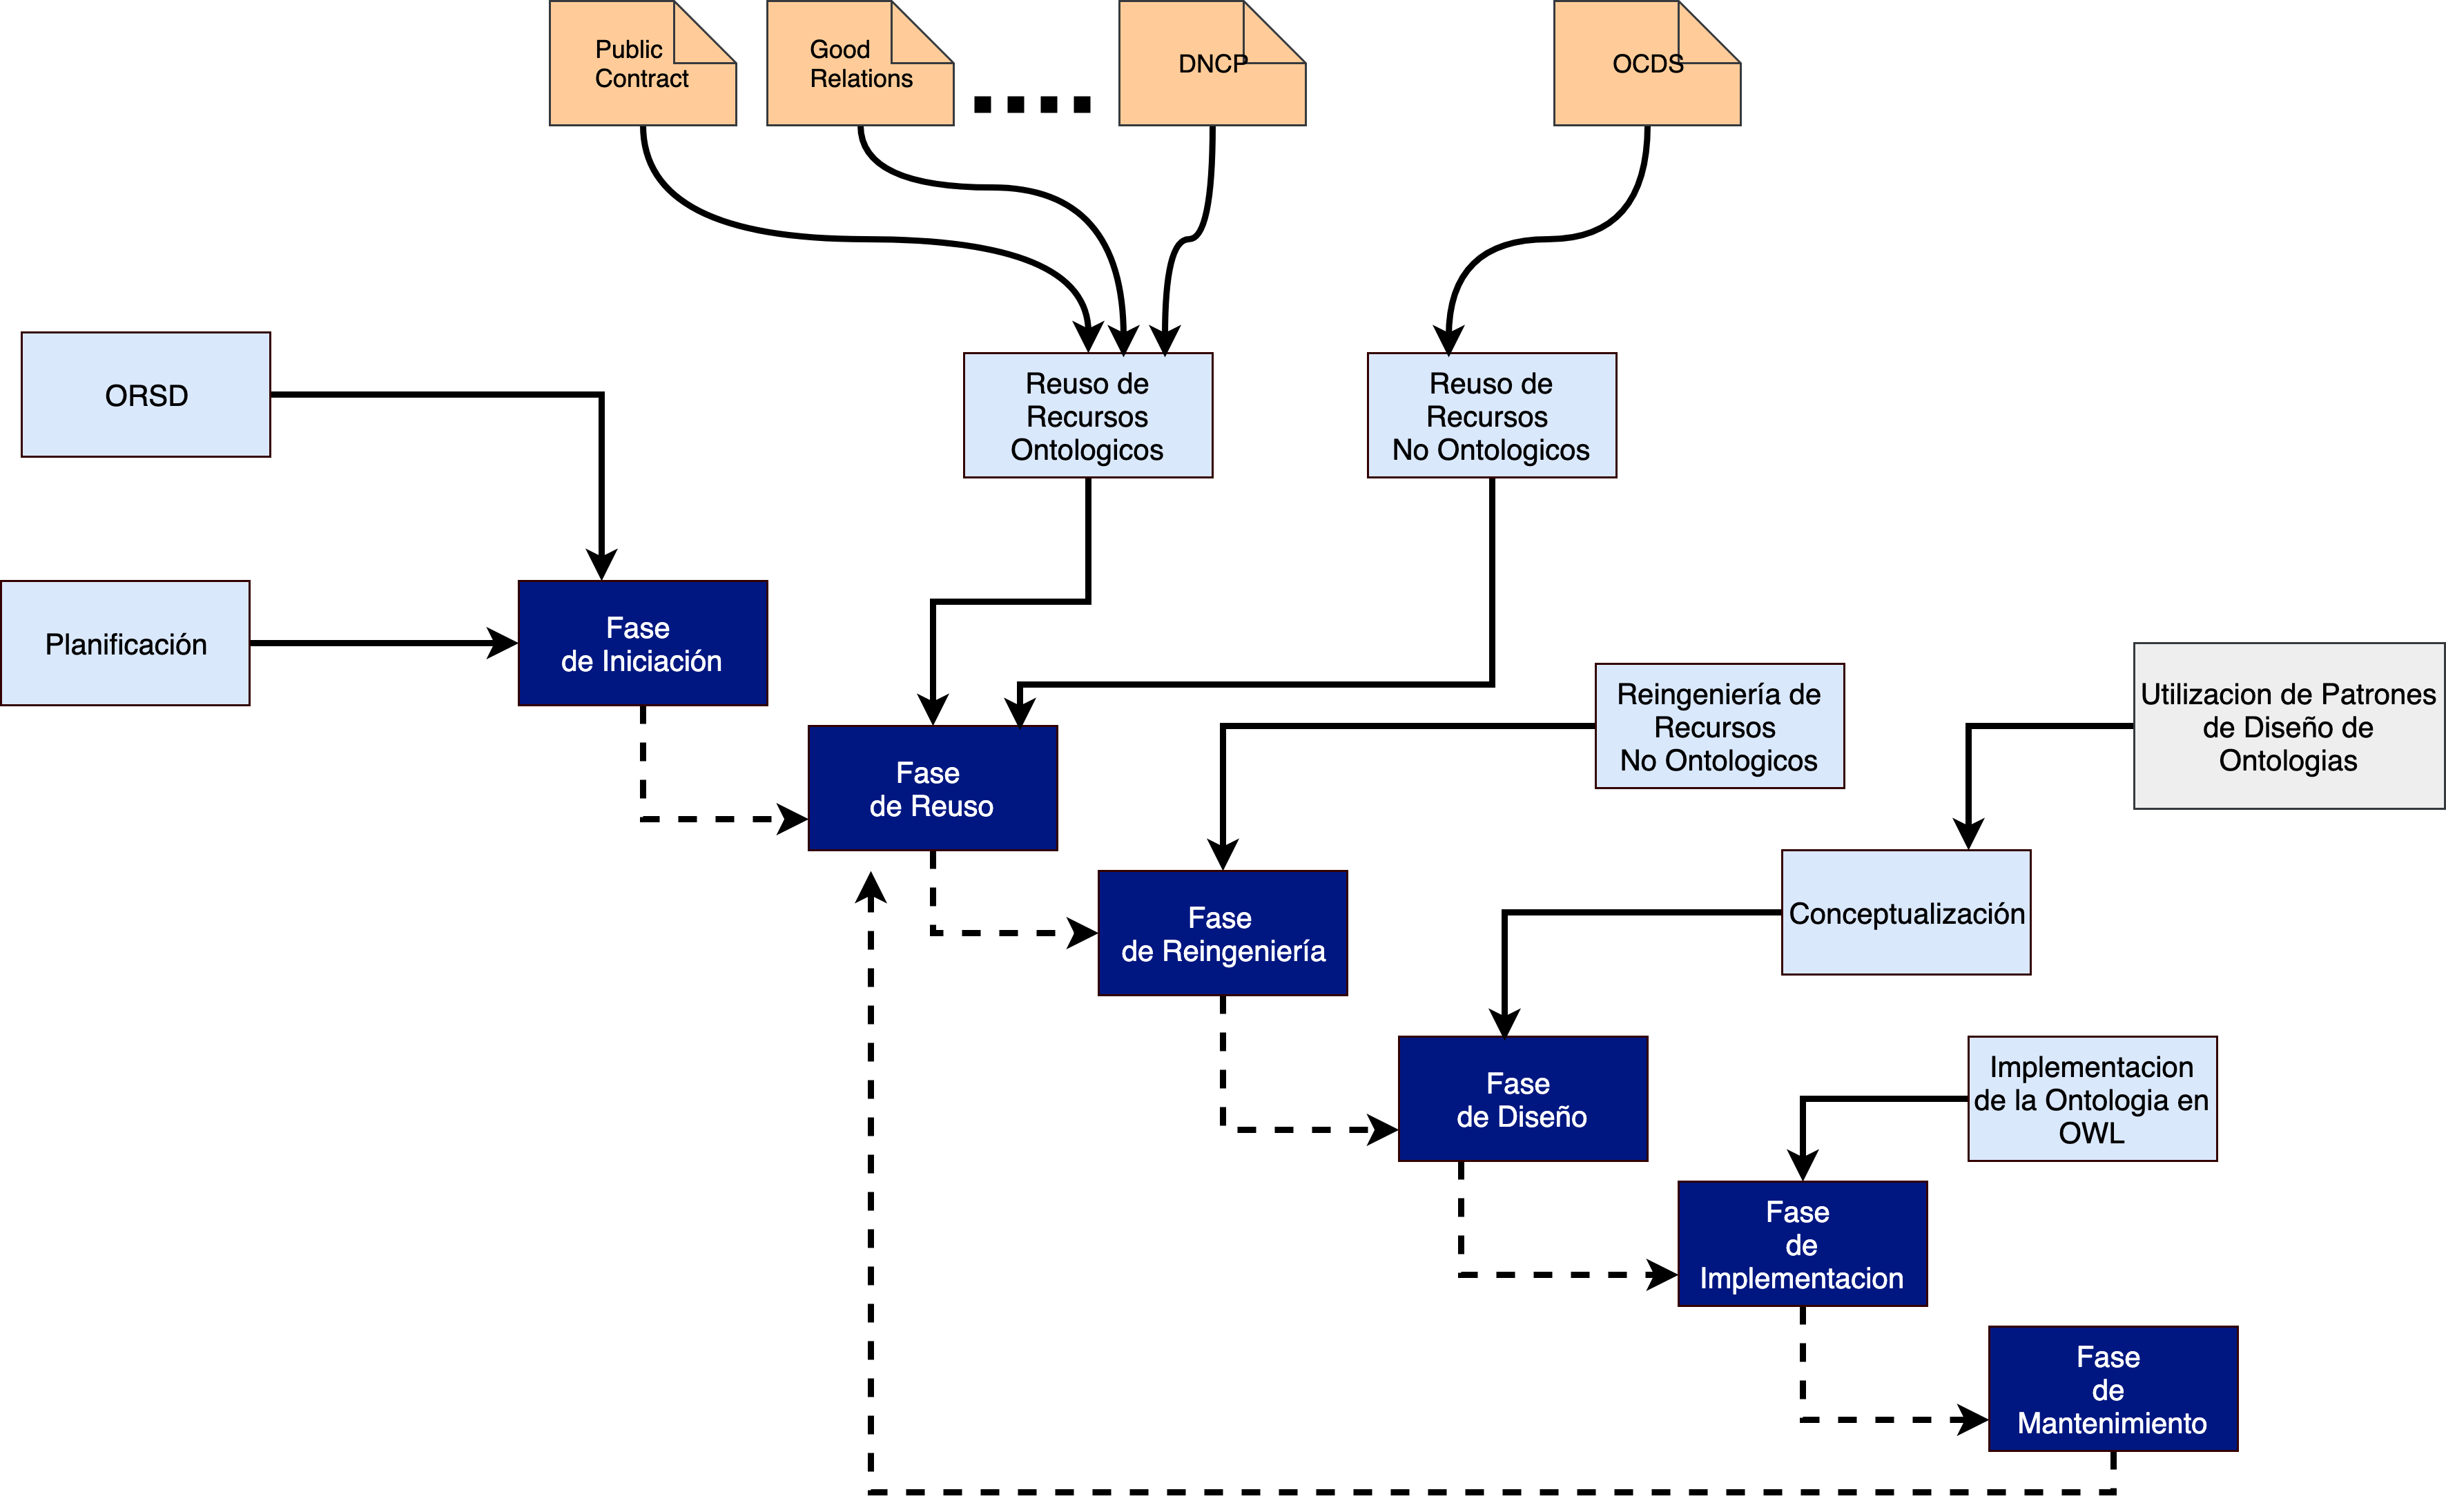
\includegraphics[width=150mm]{figuras/Diagramas-GraficodeSecuenciasDesarrollo.png}
    \caption{Modelo de Ciclo de Vida de desarrollo de la ontología.}
    \label{img:secuenciaDeDesarrollo}
\end{figure}

A continuación se citan las actividades divididas en las fases del ciclo de vida a desarrollarse según la metodología NeOn:
\begin{enumerate}
\item Fase 1: Iniciación
    \begin{enumerate}
    \item Especificación de Requerimientos Ontológicos (ORSD). Aquí se define el propósito de la ontología, su alcance, el lenguaje de implementación, el grupo objetivo, los potenciales usos de la ontología, los requerimientos funcionales y no funcionales, y un pre-glosario de términos.

    \item Planificación. Según lo expuesto en la Tabla \ref{escenarios vs modelo} se elige el modelo de ciclo de vida de 6 fases en cascada, debido a que serán necesarias las fases de reuso tanto de recursos ontológicos como no-ontológicos, reingeniería, y diseño para la implementación.
 
    \end{enumerate}
\item Fase 2: Reuso
    \begin{enumerate}
    \item Reuso de Recursos  no-ontológicos. Los recursos no-ontológicos (NOR) representan recursos de conocimiento cuya semántica no fue formalizada por una ontología. Estos NORs contienen conocimientos de un dominio en particular y representan algún grado de consenso colectivo.

    \item Reuso de Recursos Ontológicos. A fin de no redoblar esfuerzos y con la intención de integrar esta nueva ontología con otras, se procede al reuso de recursos ontológicos. En esta actividad se procedió a la búsqueda, evaluación y selección de las ontologías a reusar.
    \end{enumerate}
\item Fase 3: Reingeniería
\begin{enumerate}
\item Reingeniería de Recursos No-Ontológicos. En esta actividad se analizan posibles patrones de diseño a la hora de la implementación, así como una metodología para transformar la semántica incluida en el OCDS.

\end{enumerate}
\item Fase 4: Diseño
\begin{enumerate}
\item Conceptualización de la Ontología. En esta actividad se identifica el esquema de recursos así como también los componentes conceptuales y sus relaciones. Además, se crea un modelo conceptual dividido por bloques de conceptos relacionados. El conocimiento se expresa mediante representaciones primitivas de conceptos y relaciones entre conceptos. A continuación se representa la conceptualización teniendo como base el OCDS. 

\end{enumerate}
\item Fase 5: Implementación. En esta actividad se procede al desarrollo de la ontología utilizando la herramienta Protégé, el lenguaje utilizado fue OWL, un estándar internacional para codificar e intercambiar ontologías diseñada para la Web Semántica. 

\item Fase 6: Mantenimiento. Por último se procede a la fase del mantenimiento, que consiste en corregir o aumentar los conceptos y restricciones de la ontología para que responda a la preguntas y la detección y corrección de errores de la misma. 		

\end{enumerate}
Una vez terminada la planificación se procede al desarrollo de cada una de las demás actividades siguiendo el orden de las fases. La explicación de cada una de las actividades se describen a continuación en este documento.


\section{Reuso de recursos no-ontológicos}
Los recursos no-ontológicos (NOR)\cite{ReusoRecursoNoOntologico} representan recursos de conocimiento cuya semántica no fue formalizada por una ontología. Estos NORs contienen conocimientos de un dominio en particular y representan algún grado de consenso colectivo. Estos recursos están presentes en forma de esquemas de clasificación, tesauros, diccionarios, etc. El principal desafío de los NORs es que la semántica no siempre está formalizada, osea legible por máquina, por lo tanto no son considerados ontologías formales según la definición adoptada.

En esta sección se desarrolla la búsqueda, evaluación y selección de recursos no-ontológicos que servirán como insumo para el desarrollo de la ontología.

\subsection{Búsqueda de recursos no-ontológicos }

En el proceso de búsqueda de documentación y estándares del dominio de Contrataciones Públicas se encontró que la DNCP implementa una API utilizando el estándar de publicación de datos de contrataciones públicas internacional \textit{Open Contracting Data Standard} (OCDS). La intención de la OCP fue crear un estándar que formaliza la sintaxis y no la semántica de cada concepto, a través de JSON Schema\cite{JSONSche10:online}, que es un vocabulario que permite anotar y validar documentos JSON. El estándar posee conceptos explícitamente definidos en lenguaje natural, por ello se lo consideró un recurso no-ontológico. Cabe recordar que cuando se habla de formal, se habla de legible por máquina. 

OCDS es un estándar amigable y flexible para estructurar información de Contrataciones Públicas y es mantenido por la OCP. El estándar describe qué, cuándo y cómo disponibilizar datos y documentos asociados en las diferentes fases del proceso de contratación. El proyecto promueve la divulgación y participación en las contrataciones públicas creando un estándar abierto de datos simple. OCDS posee un esquema de datos detallado de todos los conceptos así como también la estructura de los datos divulgados, dicho esquema esta disponible el sitio web del estándar \cite{OCDSReleaseSchema:online}. Este esquema ayuda a las personas a comprender todos los campos publicados. Además el estándar posee un guía de implementación de modo a facilitar la implementación de cada país.

Se utilizó el portal de datos abiertos de la DNCP \cite{DatosAbiDNCP:online}, organismo del estado que publica datos de los procesos de contrataciones orientados a diferentes tipos de usuarios:


\begin{enumerate}
    \item Lista de datos. Con el fin de que los usuarios que necesitan ver, analizar y descargar en formato CSV los datos detallados de todos los registros de contrataciones.
    Visualizaciones de datos para usuarios que deseen ver estadísticas e información agregada.
    \item Una API para desarrolladores que permite manipular datos en formato JSON y JSON-LD de manera programática para cualquier otro uso.
    \item Plataforma de Contrataciones Electrónica, destinada a empresas y personas que deseen presentarse o conocer algún proceso de contratación.
\end{enumerate}

Los datos publicados poseen un diccionario de datos y una ontología creada por la DNCP, la cual sirve como contexto para la API desarrollada. Además la DNCP implementó una API siguiendo el estándar OCDS, que posee un esquema de publicación bien definida en JSON Schema.

\subsection{Evaluación de recursos no-ontológicos}
Se eligió el OCDS como recurso no-ontológico a evaluar puesto que el principal objetivo de este trabajo es que la ontología desarrollada sea compatible con dicho estándar de modelo de datos. Para realizar la evaluación se procedió a la extracción de las entradas léxicas, luego al cálculo de precisión y alcance para por último evaluar la factibilidad de reuso del recurso.  A continuación se explica en detalle cada paso.

\subsubsection{Extracción de entradas léxicas}
La meta de esta tarea es extraer las entradas léxicas de los recursos no-ontológicos. Para realizarla, es necesario tomar como entrada los recursos no-ontológicos y extraer sus entradas léxicas usando herramientas de extracción de terminología.	
			
Del esquema JSON de la versión 1 del OCDS se hizo una lista de todas las propiedades del mismo. Para este trabajo consideramos que cada propiedad del esquema consiste en una entrada léxica, donde una entrada léxica corresponde a un concepto o relación dentro del dominio de conocimiento. Se encontraron 142 propiedades, omitiendo las propiedades repetidas y datos transaccionales del estándar que no representan entradas léxicas, la lista se reduce a 114.

\subsubsection{Cálculo de precisión y alcance}

El objetivo de esta tarea es calcular la precisión de los recursos no-ontológicos candidatos. La precisión es una medida ampliamente utilizada en la recuperación de información y se define como la proporción del material recuperado que realmente es relevante. Esta tarea es llevada a cabo por los desarrolladores de software y los que utilicen la ontología teniendo como entrada las entradas léxicas extraídas de los recursos no-ontológicos y de la terminología reunida del ORSD. Para esto definimos los siguientes términos.

\begin{itemize}
    \item \textit{NOR Lexical Entries}  como el conjunto de entradas léxicas extraídas del recurso no ontológico.	
    \item \textit{ORSD Terminology} como el conjunto de términos identificados incluidos en el ORSD. 
\end{itemize}
Para obtener el número de términos de la especificación de requisitos de ontología (ORSDTerminology) se creó una lista unificada de todas las propiedades encontradas en el diccionario de datos del portal de datos abiertos de la DNCP.  Se encontraron 129 términos, de la misma manera que en el OCDS se omitieron propiedades repetidas y datos transaccionales, dejándonos con un total de 109 términos. Éstas representan el dominio de conocimiento que se quiere representar con la ontología a construir.

Para calcular la cobertura y la precisión del recurso no-ontológico se realizó la unión de términos equivalentes semánticamente. Dicha unión consiste en verificar términos equivalentes entre las entradas léxicas que estaban presentes en los requerimientos y en el recurso no-ontológico analizado. Cabe destacar que la metodología utilizada sólo tomó en cuenta las propiedades del esquema JSON del OCDS y el diccionario de datos de la API desarrollada por la DNCP, esto limita la cobertura, que podría ser más amplia si consideramos todos los términos del dominio de conocimiento. El resultado arrojó que existen 65 entradas léxicas comunes. Con estos datos se puede calcular la cobertura y la precisión a través de las  fórmulas \ref{eq:1} y \ref{eq:2}.

\begin{equation}
    \label{eq:1}
    Precision =  \frac{{NORLexicalEntries}*{ORDSTerminology} }{{NORLexicalEntries}}    
\end{equation}

\begin{equation}
    \label{eq:2}
     Coverage = \frac{{NORLexicalEntries}* {ORDSTerminology}}{{ORDSTerminology}}   
\end{equation}

Esto da una cobertura de 0.59 y una precisión de 0.57. 

\subsection{Evaluación y selección del recurso no-ontológico}

Como se puede ver en el esquema del OCDS\footnote{http://standard.open-contracting.org/latest/en/schema/release/}, el mismo posee una especificación formal de la sintaxis de cada una de las propiedades, ya que por medio de un validador construido por la OCP\footnote{http://standard.open-contracting.org/validator/} podemos verificar si el objeto validado cumple con los requerimientos sintácticos de publicación del estándar.

También podemos observar que el estándar contiene explícitamente las descripciones de cada una de las propiedades del esquema JSON, por lo que posee información valiosa y consensuada de cada uno de los conceptos del dominio. Sin embargo, dicha información solamente es entendible por personas, no así procesable por máquinas, por lo que representa un recurso no-ontológico vital para el desarrollo de nuestra ontología.

Como se puede ver en el esquema del OCDS, el mismo posee una especificación formal de la sintaxis de cada una de las propiedades, ya que por medio de un validador construido por la OCP podemos verificar si el objeto validado cumple con los requerimientos sintácticos de publicación del estándar.

También podemos observar que el estándar contiene explícitamente las descripciones de cada una de las propiedades del esquema JSON, por lo que posee información valiosa y consensuada de cada uno de los conceptos del dominio. Sin embargo, dicha información solamente es entendible por personas, no así procesable por máquinas, por lo que representa un recurso no-ontológico vital para el desarrollo de nuestra ontología.



Las principales diferencias de cobertura entre los conceptos de la DNCP y la OCDS son que el segundo posee mayor información como es el caso de Periodo, Organización y Detalle de Contacto. También contempla los conceptos de Documentos, Transacciones, Hitos, una fase adicional de Implementación del Contrato y guarda el historial de cambios de todas las propiedades a través de las Adendas. Así también, el dominio de la DNCP agrega conceptos como Modificaciones de Contrato e información más detallada de Proveedores y Convocatorias. En la figura \ref{img:coberturaontologia} se aprecia la intersección de los principales conceptos entre ambos dominios de conocimientos.

\begin{figure}[ht!]
    \centering
    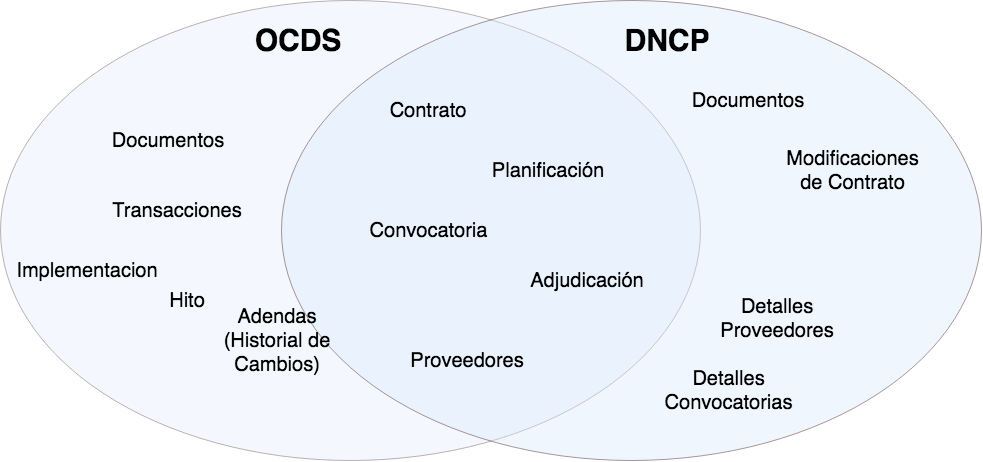
\includegraphics[width=150mm]{figuras/Diagramas-VennCobertura.png}
    \caption{Cobertura de los terminos de la DNCP y la OCDS}
    \label{img:coberturaontologia}
\end{figure}

    

El OCDS es implementado a nivel internacional, tiene una comunidad de colaboradores expertos en el dominio de distintos países, implementadores que dan al estándar una validez en cuanto a la aceptación de los términos, posee listas de correos y un sistema de gestión de cambios y mejoras activo en la plataforma Github\footnote{https://github.com/open-contracting/standard}. La intención de este trabajo es que la ontología sea utilizada no solamente sea utilizada por la DNCP sino por cualquier ente que realice procesos licitatorios, además, la DNCP está utilizando este estándar para publicación de datos orientados a desarrolladores. Con todo esto se aprecia que la cobertura es suficiente para utilizar el OCDS como recurso no-ontológico para nuestra ontología sacrificando así algunos detalles específicos de implementación local. Estos detalles más específicos se podrían cubrir a través del reuso y extensión de la ontología desarrollada en un futuro trabajo.

\section{Reingeniería de recurso no-ontológicos}
Debido a que se utilizó recursos no-ontológicos, debemos de realizar un proceso de reingeniería para transformar estos recursos de manera a incluir esa información en la ontología. Procedemos de esta manera al proceso de reingeniería del esquema de publicación de OCDS.


\subsection{Ingeniería reversa del recurso no-ontológico}
El primer paso es analizar el recurso no-ontológico para identificar los principales componentes y crear representaciones del recurso. Dentro de esta actividad procederemos a la recolección de los datos, la abstracción conceptual y exploración de la información.

\subsubsection{Recolección de datos}

El propósito de esta actividad es buscar y recolectar todos los datos y la documentación del recurso no-ontológico incluyendo su propósito, componentes, modelo de datos y detalles de implementación.

El OCDS es un estándar abierto de datos para la publicación de información estructurada sobre todas las etapas de un proceso de contratación: desde la planificación hasta la implementación.

La publicación de los datos siguiendo el OCDS permite una mayor transparencia en la contratación pública y puede apoyar al análisis accesible y a profundidad de la eficiencia, efectividad, equidad e integridad de los sistemas de contratación pública. El OCDS fue diseñado con un enfoque en la contratación pública de bienes, obras y servicios, pero puede ampliarse para su uso en otros contextos. 

El OCDS se centra en las siguientes necesidades del usuario:
\begin{itemize}
    \item Fortalecimiento de la transparencia, rendición de cuentas e integridad de los contratos públicos.
    \item Hacer un buen uso del dinero del gobierno.
    \item Permitir al sector privado una competencia justa por contratos públicos.
    \item Control de la eficacia de la prestación de servicios. 
\end{itemize}

El OCDS posee un sitio web donde se encuentra documentado todo el estándar, soportando los idiomas español, inglés y francés. Además posee una guía de implementación del estándar, un validador de la estructura sintáctica del mismo y un mecanismo de gestión de extensiones.

\subsubsection{Modelo conceptual}

En esta actividad se identifica el esquema de recursos así como también los componentes conceptuales y sus relaciones. Además se crea un modelo conceptual dividido por bloques de conceptos relacionados. El conocimiento se expresa mediante representaciones primitivas de conceptos y relaciones entre conceptos. A continuación se representa la conceptualización teniendo como base el OCDS.

Un proceso de contratación se define como toda la información relativa a la planificación, la licitación, las adjudicaciones, los contratos y la ejecución de contratos relacionados con un solo proceso de iniciación.

Un proceso de contratación agrupa información sobre diferentes etapas o fases relacionadas a la vida útil de un contrato, a partir de la planificación, progresando a través de las etapas de iniciación u oferta, luego por la adjudicación y contrato y finalizando con la implementación del producto o servicio como se muestra en la Figura \ref{img:fases del proceso licitatorio }.

\begin{figure}[!htbp]
    \centering
    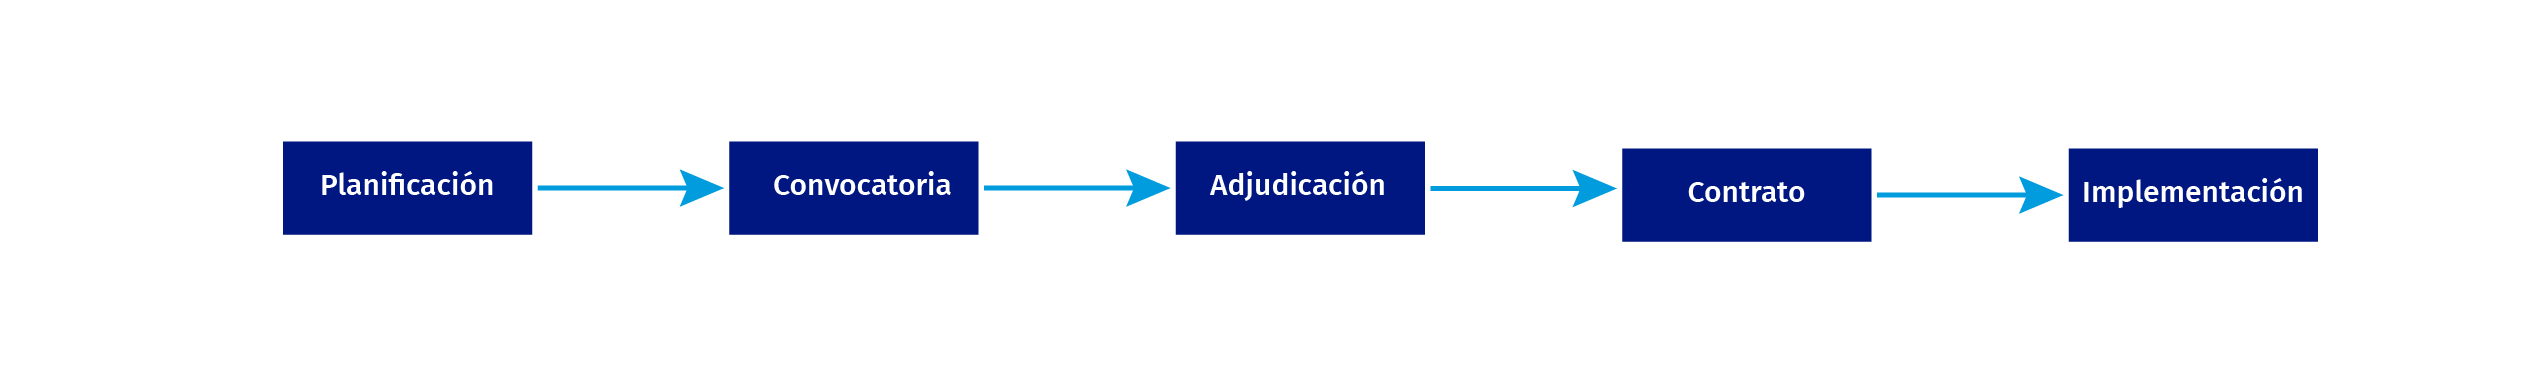
\includegraphics[width=150mm]{figuras/Diagramas_ProcesoLicitatorio.png}
    \caption{Modelo de fases del Proceso Licitatorio}
    \label{img:fases del proceso licitatorio }
\end{figure}

Las etapas son correlativas, esto significa que necesariamente debe de existir la etapa anterior antes de existir la siguiente. Todas las etapas representan un bloque de información.

Además de estas etapas existe otro concepto importante que es el bloque de Organización, que puede corresponder tanto al comprador como al oferente. Esta Organización puede estar ligada a cualquiera de las etapas del proceso de contratación. A continuación se detallan cada una de las etapas.
\paragraph{Planificación (\textit{Planning})}\hfill \break
Este bloque contiene información necesaria para describir los antecedentes de un proceso de contratación y puede incluir detalles del presupuesto del que se extraen los fondos o proyectos relacionados. Todo proceso de contratación posee una única planificación, dicha planificación tiene un presupuesto (budget) asociado donde finalmente se indica el valor o monto estimado para la adquisición del bien o servicio. Un diagrama de los componentes principales de la clase Planificación puede verse en la Figura \ref{img:Fase de Planificacion}.

\begin{figure}[htbp!]
    \centering
    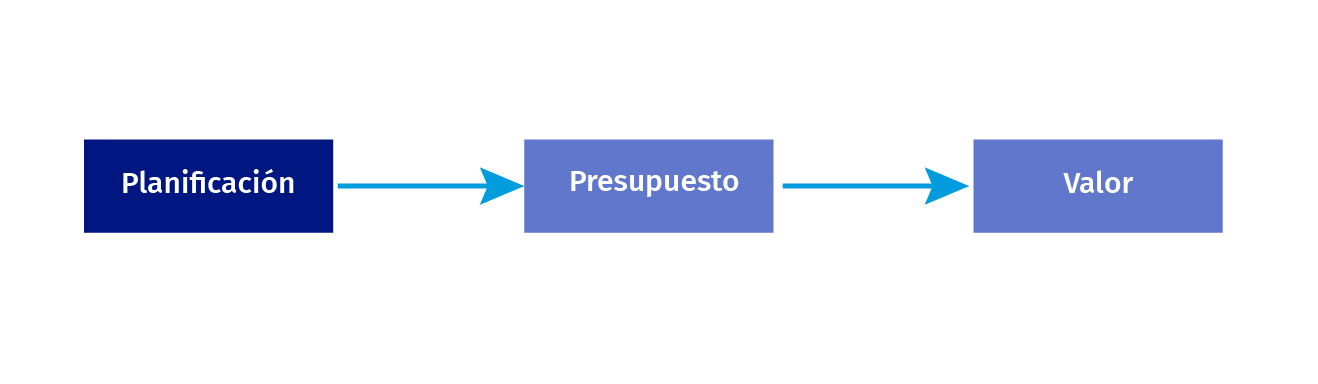
\includegraphics[width=150mm]{figuras/Diagramas_Planificacion.png}
    \caption{Modelo de fase de Planificación}
    \label{img:Fase de Planificacion}
\end{figure}

\paragraph{Convocatoria (\textit{Tender})}\hfill \break
Este bloque incluye detalles del anuncio indicando que una organización tiene la intención de abastecerse de algunos bienes o servicios y establecer uno o más contratos para estos. Todo proceso de contratación posee una única convocatoria, dicha convocatoria tiene asociada la organización involucrada en el proceso. Además, la convocatoria indica los ítems requeridos, el período establecido, los documentos utilizados, las adendas que pudieran haberse realizado sobre la convocatoria original y la lista de hitos. Se observa el esquema en la Figura \ref{img:Fase de Convocatoria}

\begin{figure}[htbp!]
    \centering
    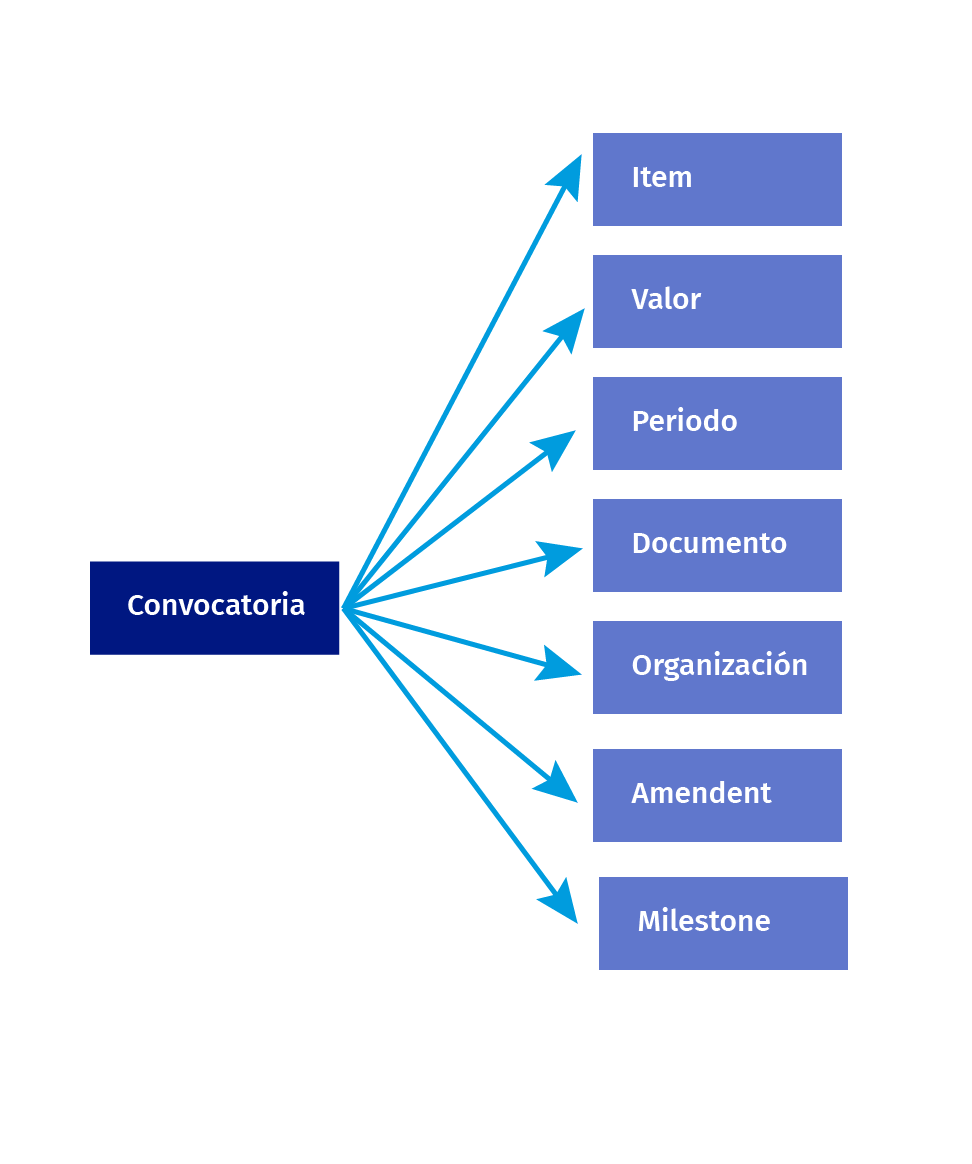
\includegraphics[width=150mm]{figuras/Diagramas_Convocatoria.png}
    \caption{Modelo de fase de Convocatoria}
    \label{img:Fase de Convocatoria}
\end{figure}

\paragraph{Adjudicación (\textit{Award})}\hfill \break
Este bloque se utiliza para anunciar las adjudicaciones emitidas para una licitación. Todo proceso de contratación puede involucrar una o más adjudicaciones, dichas adjudicaciones indican, para cada proveedor (organización), los ítems adjudicados, el valor o monto adjudicado y los documentos asociados al proceso. Esto se aprecia en la Figura \ref{img:Fase de Adjudiacion}


\begin{figure}[htbp!]
    \centering
    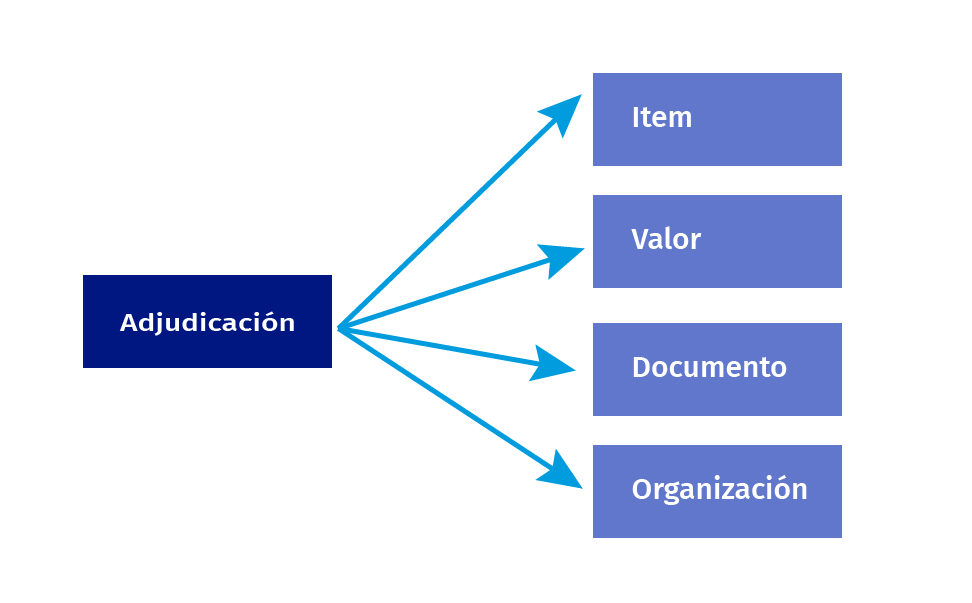
\includegraphics[width=150mm]{figuras/Diagramas_Adjudicacion.png}.
    \caption{Modelo de fase de Adjudicación}
    \label{img:Fase de Adjudiacion}
\end{figure}


\paragraph{Contrato (\textit{Contract})}\hfill \break
Este bloque se utiliza para proporcionar detalles de los contratos que se han celebrado. Todo proceso de contratación puede involucrar uno o más contratos, cada uno de los cuales debe estar asociado a una adjudicación específica. El proveedor (organización) adjudicado está indicado en la adjudicación, no así en el contrato. El contrato también indica los ítems adjudicados, los documentos asociados al proceso y la implementación del contrato. La implementación del contrato contiene información acerca de los hitos, las transacciones realizadas y los documentos utilizados. En la Figura \ref{img:Fase de Contrato} vemos un esquema de la estructura del Contrato.

\begin{figure}[htbp!]
    \centering
    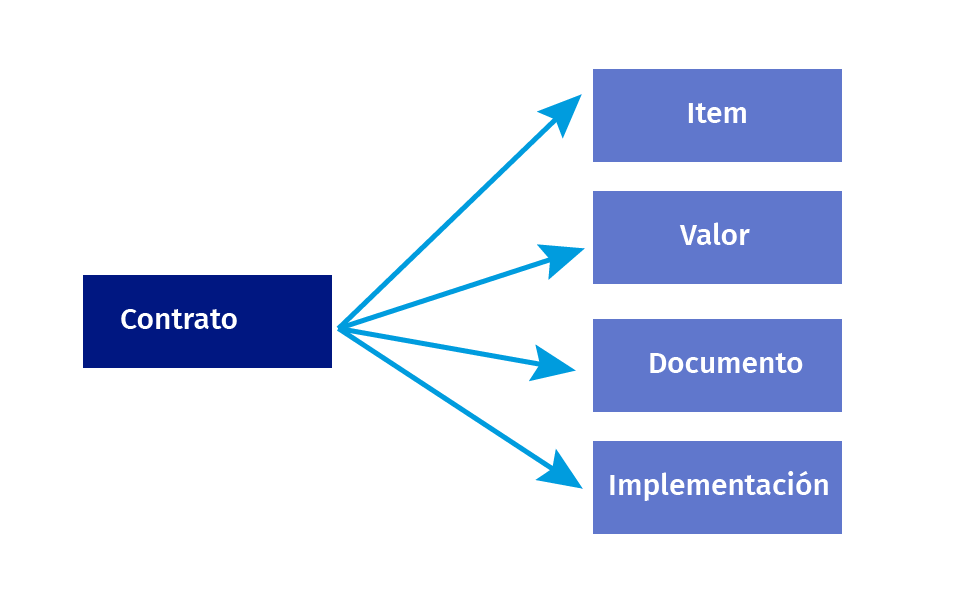
\includegraphics[width=150mm]{figuras/Diagramas_Contrato.png}
    \caption{Modelo de fase de Contrato}
    \label{img:Fase de Contrato}
\end{figure}

\paragraph{Otros componentes del estándar}\hfill \break
El estándar posee además otros componentes o bloques que agrupan y contienen metadatos de publicación de los datos.  A continuación se detallan dichos componentes.

\paragraph{\textit{Releases}}\hfill \break
Para fomentar la mayor apertura de información el estándar está preparado para publicar la información en tiempo real. En cada etapa del proceso de contratación o con cada cambio que ocurra sobre los datos, el estándar prevé la publicación de esa nueva porción de información mediante releases.
Los releases son acumulativos, es decir, durante un proceso de contratación se pueden proporcionar uno o más releases, por ejemplo: describir una licitación, anunciar la adjudicación de contratos y proporcionar actualizaciones sobre los mismos.
Una vez que un release ha sido publicado no puede cambiar. La información actualizada debe ser compartida a través de un nuevo release.
Los releases pueden ser publicados a través de un único sistema o de manera distribuida por diferentes sistemas, pero todos éstos deben estar relacionados a partir de un identificador único denominado Open Contracting ID (OCID).

\paragraph{\textit{Releases}}\hfill \break
Un registro (\textit{Record}) de contratación provee una instantánea del proceso de contratación en un punto dado en el tiempo, que reúne todas las versiones por las cuales pasó ese proceso en un solo lugar.
Un Record contiene tres elementos clave: 
\begin{itemize}
    \item Una lista de todos los releases asociados a un proceso de contratación en particular, 
    \item Un release compilado que contiene la última versión de los datos,
    \item Una versión histórica de releases que contiene la historia con todos los cambios realizados sobre los datos.
\end{itemize}

\paragraph{\textit{Release package}}\hfill \break
Un release package es un esquema de agrupación para la publicación de releases, describe el documento contenedor y metadatos para la publicación de releases.

\paragraph{\textit{Record package}}\hfill \break
Un Record Package es un esquema de agrupación para la publicación de Records, describe el documento contenedor y metadatos para la publicación de Records. En la Figura \ref{img:Record Package} se muestra el modelo conceptual de \textit{Record Package}.



\begin{figure}[ht!]
    \centering
    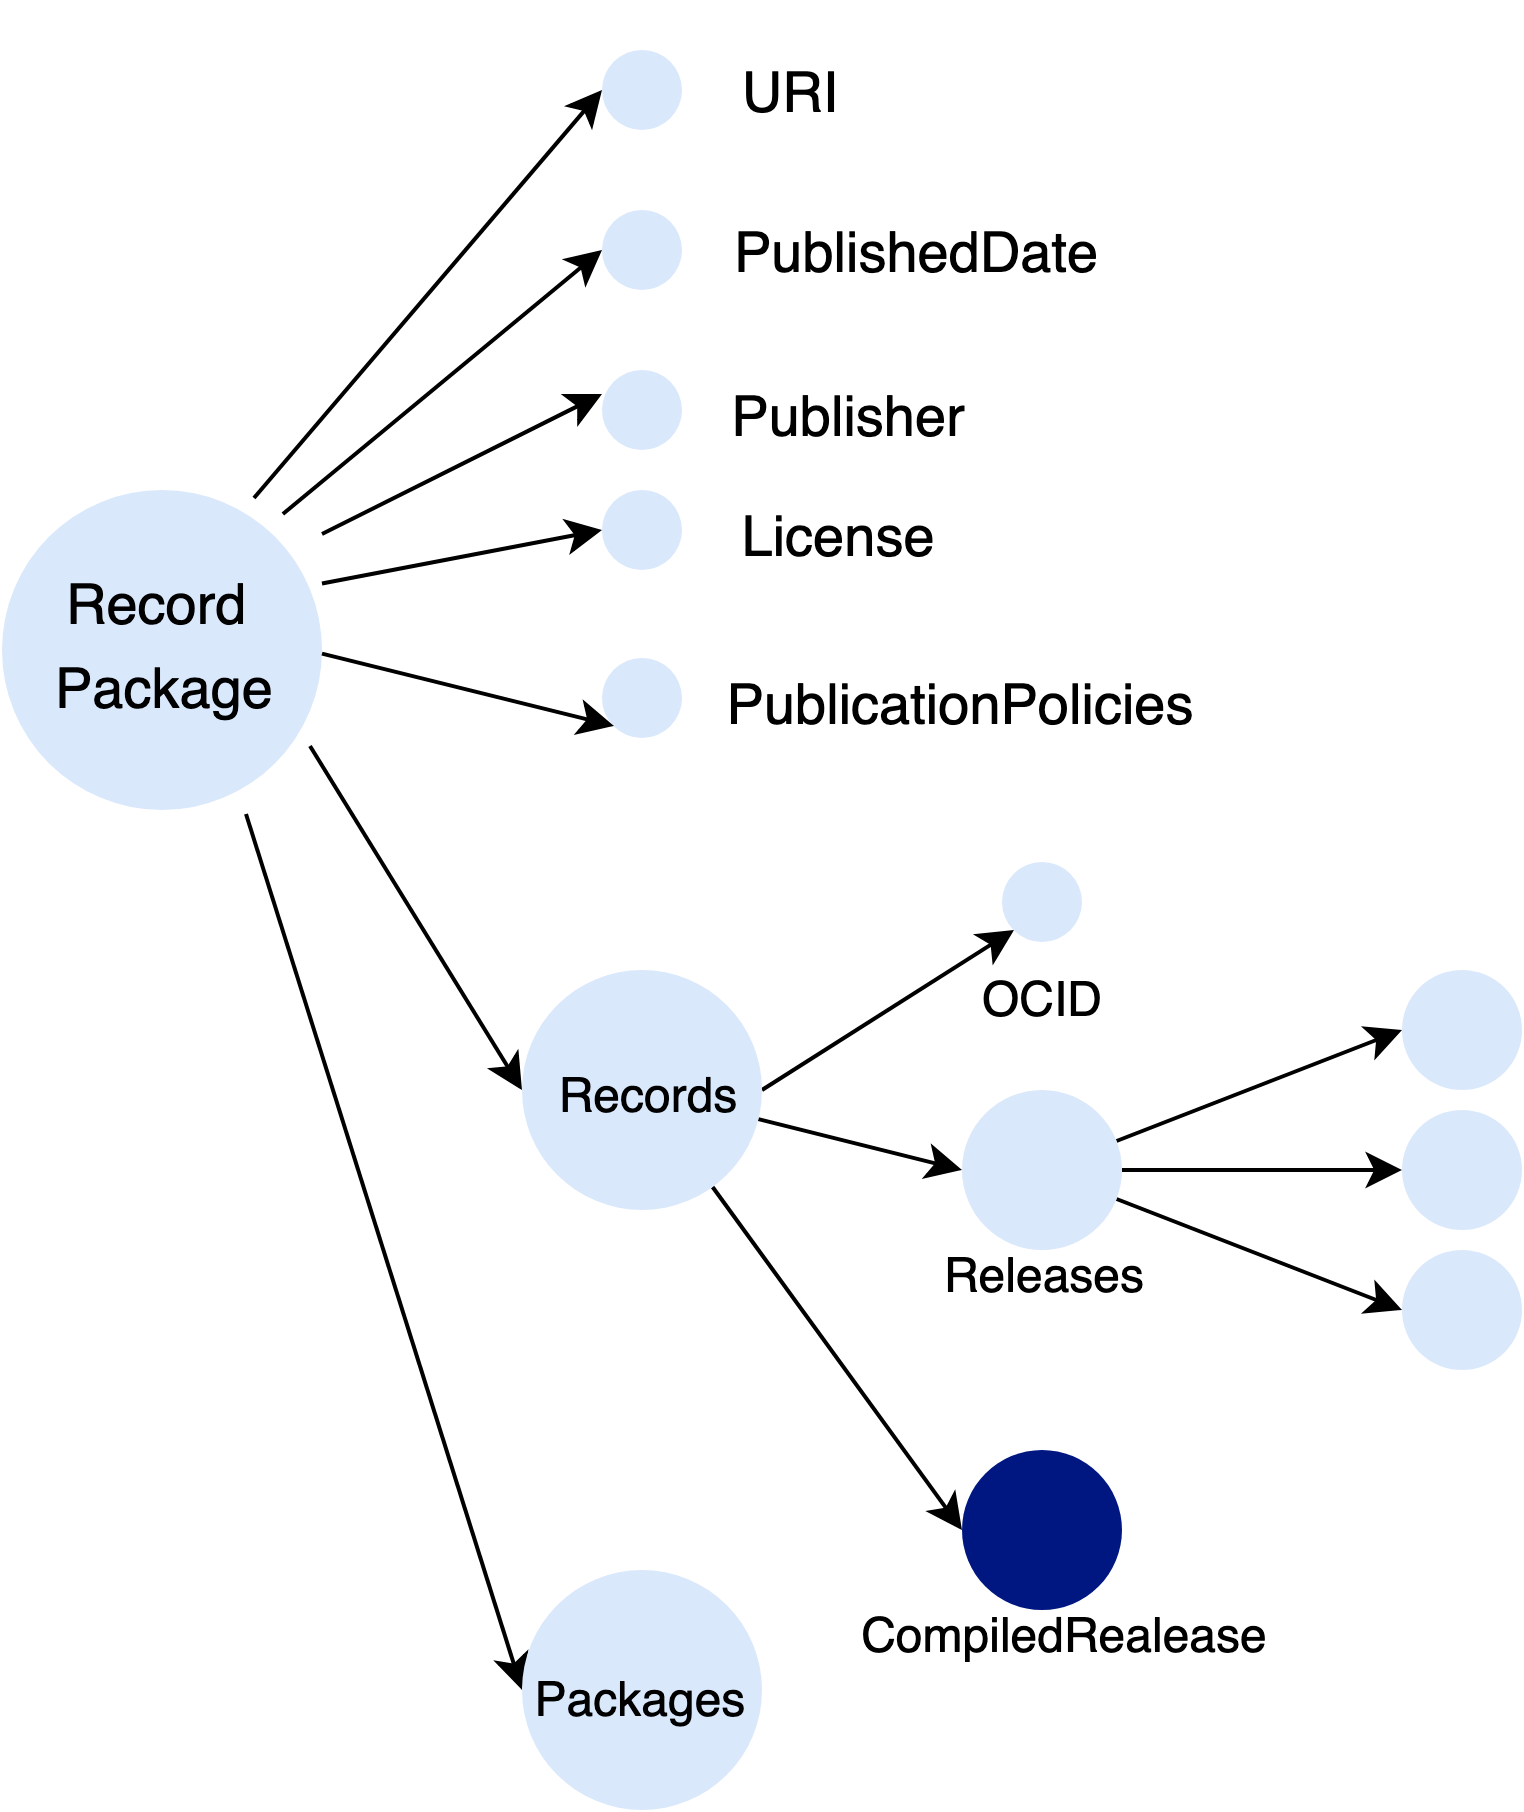
\includegraphics[width=150mm]{figuras/Diagramas-RecordPackage.png}
    \caption{Record Package}
    \label{img:Record Package}
\end{figure}


\subsubsection{Transformación del recurso no-ontológico}
En esta sección se utilizaron los patrones de diseño para seguir construyendo un modelo conceptual y luego proseguir con la implementación de la ontología. 
\paragraph{Búsqueda de Patrones de Diseño}\hfill \break
El objetivo de este paso es buscar posibles patrones de diseño que conviertan el recurso no-ontológico en un modelo conceptual. 
Una vez analizado el esquema del OCDS se procedió a la búsqueda de patrones de diseño de ontologías, se utilizó el repositorio ontologydesingpatterns.org para realizar esta búsqueda de patrones bien conocidos por la comunidad de desarrolladores de ontologías y recomendado por la metodología NeOn.
Los patrones que son relevantes son aquellos que involucran tiempo, dinero, empresas u organizaciones, lugares y procesos en general. Luego de una búsqueda se encontraron los siguientes patrones de diseño que podrían ser útiles al momento del desarrollo de la ontología.
\begin{enumerate}
    \item Intervalo de tiempo\footnote{http://ontologydesignpatterns.org/wiki/Submissions:TimeInterval}
    \item Precio\footnote{http://ontologydesignpatterns.org/wiki/Submissions:Price} 
    \item Etiquetas\footnote{http://ontologydesignpatterns.org/wiki/Submissions:Tagging}
    \item Lugar\footnote{http://ontologydesignpatterns.org/wiki/Submissions:Place}
    \item Lista\footnote{http://ontologydesignpatterns.org/wiki/Submissions:List}
    \item Secuencia\footnote{http://ontologydesignpatterns.org/wiki/Submissions:Sequence}
    \item Boleta de Pago\footnote{http://ontologydesignpatterns.org/wiki/Submissions:Invoice} 
\end{enumerate}

Además se investigaron otros patrones de reingeniería, pero ninguno de éstos se adecuaba ya que están orientados a patrones jerárquicos de diseño y el dominio modela una secuencia o proceso. 

Se creó un patrón de conversión del estándar de documentacion JSON SCHEMA http://json-schema.org/ a un modelo ontológico. El patrón de conversión tiene los siguientes lineamientos.

\begin{itemize}
    \item Todos los objetos JSON del esquema son potenciales conceptos de la ontología desarrollada. Un Objeto JSON será considerado como clase o individuo en el modelo conceptual.
    \item El hecho de que un objeto esté relacionado a otro no necesariamente indica una relación de jerarquía, puede a la vez tratarse de una relación de contención, uso, correlación o dependencia.
    \item Todos los atributos de un Objeto JSON de tipo \textit{string} o numérico son potenciales propiedades (en la ontología) del concepto generado a partir el Objeto JSON.
    \item Los tipos de datos nos indican el tipo de dato en el formato RDF. Por ejemplo, si dentro de JSON Schema tenemos un campo que solo acepta números, podemos decir que esa propiedad es de tipo \textit{xsd:long}. Así, pueden ser una restricción en los valores de la propiedad.
    \item El nombre del objeto JSON es un candidato para nombrar esta relación. Por ejemplo, un presupuesto posee un objeto de nombre monto, de tipo valor. Por lo que podemos decir que el nombre de la relación entre presupuesto y valor se llamará monto.
    \item Los arreglos son representados a través de la relación uno a muchos dentro del modelo ontológico.
    \item Los atributos \textit{id}, \textit{identifier} o similares son potenciales identificadores de las instancias de cada concepto.
    
\end{itemize}

El esquema del OCDS posee una lista de códigos (\textit{Codelist}) de dos tipos, abiertos y cerrados. Los \textit{Codelist} Abiertos proveen códigos sugeridos, los publicadores pueden extender esta lista con nuevos códigos sin el consenso de otros publicadores. Mientras que los \textit{Codelist} Cerrados proveen códigos mandatorios, los publicadores solo pueden utilizar los valores de la lista oficial, cambios a \textit{Codelist} cerrados deben hacerse a través de la gobernanza y revisión de la lista. Esta lista de códigos fueron transformados utilizando el patrón mencionado a continuación. 

Para los \textit{Codelist} Abiertos se los convirtió en \textit{individuals}, en otros términos, instancias de los conceptos. Para los \textit{Codelist} Cerrados  se los convirtió en \textit{Enumerated Classes}. Las \textit{Enumerated Classes} impiden la declaración de nuevos individuos que pertenecen a esta clase, siendo así más restrictivos.
\paragraph{Utilización de patrones}\hfill \break
Por último, se consideraron los patrones mencionados anteriormente para los siguientes conceptos:
Para el concepto \textit{Value} del OCDS, que representan valores monetarios, se utilizó el patrón \textit{Price}. El patrón describe el precio de alguna entidad, dicho precio contiene un valor y una moneda. En la Figura \ref{img:Modelo de Precio} se muestra el diagrama del patrón.

\begin{figure}[ht!]
    \centering
    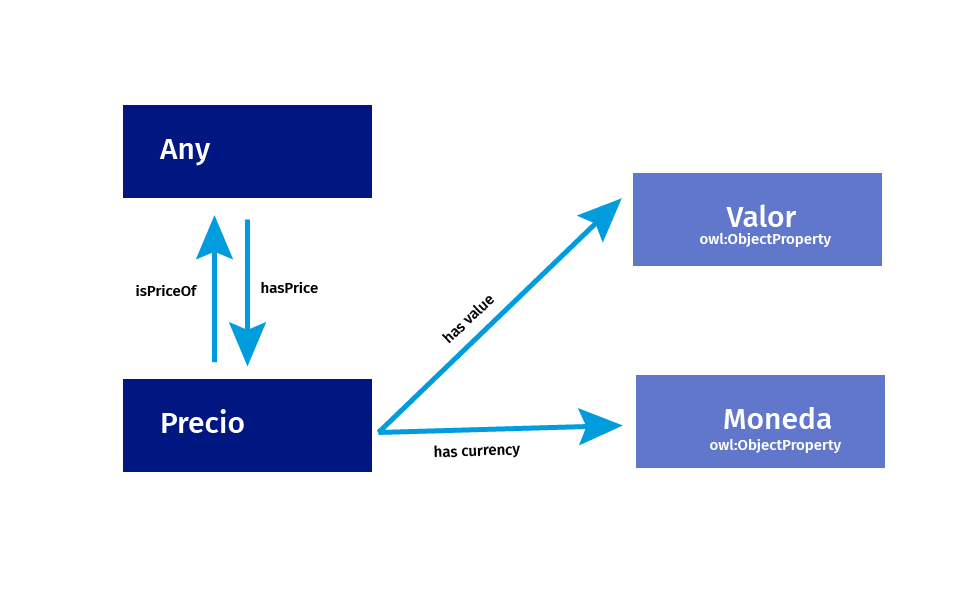
\includegraphics[width=150mm]{figuras/Diagramas_Precio.png}
    \caption{Modelo de Precio}
    \label{img:Modelo de Precio}
    
\end{figure}

En cuanto a la implementación, se optó por mantener \textit{Value} y \textit{Currency} como \textit{DataType properties} para mantener la simplicidad de nuestra ontología.

Para el concepto \textit{Period}, que representan periodos de tiempo se utilizó el patrón \textsc{Time Interval}. El patrón describe un intervalo de tiempo que contiene una fecha de inicio, una fecha de fin y una fecha del intervalo. Un posible uso del patrón sería la fecha “Agosto del 2018” tiene un fecha de inicio “1 de Agosto” y una fecha de fin “31 de Agosto”. En la implementación se omitió la propiedad Intervalo de tiempo, ya que no es necesaria para este este dominio. El modelo se puede ver en la Figura \ref{img:Modelo de Intervalo de precio}.

\begin{figure}[ht!]
    \centering
    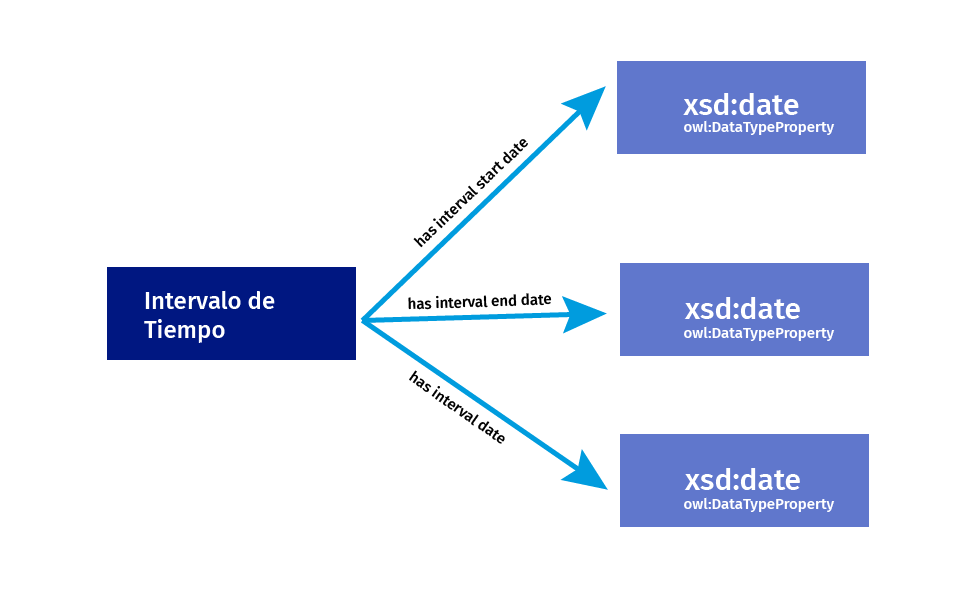
\includegraphics[width=150mm]{figuras/Diagramas_Tiempo.png}
    \caption{Modelo de Intervalo de tiempo}
    \label{img:Modelo de Intervalo de precio}
    
\end{figure}

Para la relación que existe entre \textit{Planning, Tender, Award, Contract e Implementation}, que tienen una relación de dependencia y de secuencia, se utilizó el patrón \textit{Sequence}. El patrón describe una secuencia de hecho a través de las propiedades Precede, Precede Directamente, Antecede y Antecede Directamente. Por ejemplo, decidir qué camisa utilizaré precede directamente a colocarse la camisa, y precede a colocarse la corbata. En la Figura \ref{img:Modelo de dependencia y secuencia} se presenta el diagrama del patrón. Se utilizó este patrón para describir la secuencia del proceso de contrataciones.

\begin{figure}[ht!]
    \centering
    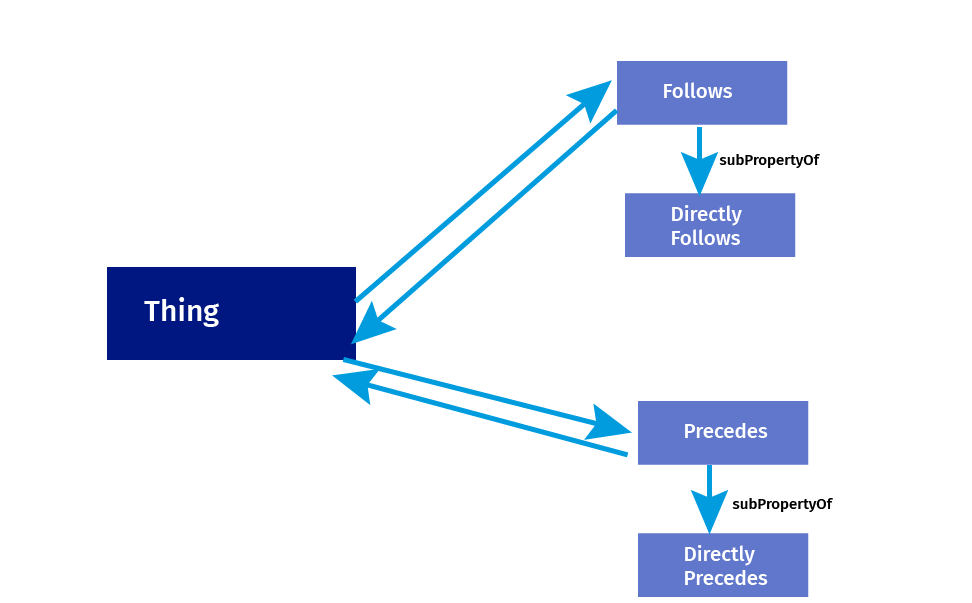
\includegraphics[width=150mm]{figuras/Diagramas_Follows.png}
    \caption{Modelo de dependencia y secuencia}
    \label{img:Modelo de dependencia y secuencia}
    
\end{figure}

\subsubsection{Construcción de la ontología}

Una vez concluido el modelo conceptual de la ontología procedemos a la construcción de la misma utilizando el lenguaje OWL y la herramienta Protégé.

Dentro de la fase de búsqueda de recursos Ontológicos, se encontró una ontología desarrolladas\footnote{https://github.com/ColinMaudry/open-contracting-ld} por un colaborador al proyecto OCD, la ontología siguió una transformación directa de JSON SCHEMA del estándar, la misma representa un punto de partida para seguir desarrollando la ontología. De esta manera además queremos incentivar la colaboración y hacer partícipe a toda la comunidad del OCDS.

El primer paso fue importar la ontología al software Protégé. Al hacer esto el software reestructuró el código de la ontología e hizo inferencias básicas detalladas a continuación. La estructura del documento del cual se partió estaba agrupada según conceptos semánticos relacionados. Protégé estructuró la ontología según sean \textit{Annotation Property, DataType Property u Object property} y luego ordenó de forma alfabética tomando como referencia el nombre de la propiedad.

Se encontraron algunas inconsistencias sintácticas dentro de la ontología, debido a que la misma fue hecha sin utilizar ninguna herramienta para desarrollo de ontologías, lo cual da lugar a errores sintácticos. Por ejemplo, el rango de la clase \textit{FormerValue} estaba definido como \textit{xsd:Integer}, Protégé infiere de que se trataba de un nuevo tipo de dato,  debido a que no existe este tipo de dato sino que debe ser \textit{xsd:integer}. Así también otro error en el documento en donde se escribió \textit{commnent} en lugar de \textit{commnent}, inmediatamente Protégé infiere como un nuevo tipo de dato. Como aprendizaje, el uso de una herramienta ontológica como Protégé nos ayuda a prevenir errores de sintaxis en la creación de la ontología y además acelera el proceso de desarrollo gracias a una interfaz gráfica que nos ayuda a distinguir entre Clases, \textit{DataType Properties} por citar algunas funcionalidades.

Toda la ontología inicial utilizó el tipo \textit{rdf:Property} para definir las propiedades. Debido a que \textit{owl:ObjectProperty} y \textit{owl:DataTypeProperty} son subclases de \textit{Property}, se decidió especializar las relaciones con estas subclases. Las propiedades que relacionan dos instancias fueron asignadas como owl:ObjectProperty y las propiedades relacionadas entre una instancia y un valor fueron asignadas como owl:DataTypeProperty.

Una propiedad de objeto (\textit{ObjectProperty}) se utiliza para conectar pares de individuos a través de IRIs, mientras que una propiedad de tipo de dato (\textit{DataTypeProperty}) relaciona una instancia de una clase con un literal.

Una propiedad funcional (\textit{FunctionalProperty}) es una propiedad que solamente puede tener un valor Y por cada instancia X, por ejemplo no puede haber dos valores distintos Y1 e Y2 tal que los pares (X,Y1) y (X,Y2) sean instancias de esta propiedad. Tanto los “ObjectProperty” como los \textit{DataTypeProperty} pueden ser declarados como \textit{DataTypeProperty}.


Una consideración importante es que para los \textit{DataType Properties} no es necesario definir como la propiedad functional ya que la mayoría de los motores de razonamiento pueden deducir que dos literales son distintos. Ejemplo: un razonador puede inferir que  el literal “1” es distinto que  "2".

El motor de inferencia agregó un axioma indicando que rdf:descriptions es igual a \textit{owl:AnnotationProperty}, que es una manera de anotar información descriptiva de la propiedad. Además se utilizó la propiedad \textit{rdf:Resource}, clase que no existe en en el estándar RDF, debería indicar la clase RDFS \textit{ rdfs:Resource} para indicar hipervínculos. En este caso se vió que semánticamente se adecua mejor la propiedad \textit{DCTERMS:URI}.

Así, se pudo construir la ontología base partir de un recurso No-Ontológico como ser el Open Contracting Data Estándar. En el siguiente apartado se abocará a la búsqueda y reutilización de recursos Ontológicos para enriquecer la ontología desarrollada.


\section{Reuso de Recursos Ontológicos}
Los pasos para el reuso de una ontología son la búsqueda, análisis y comparación de ontologías desarrolladas y luego la selección e integración de las ontologías a reutilizar. Al mismo tiempo existen distintas maneras de reutilizar una ontología, como veremos más adelante. 

\subsection{Búsqueda de Ontologías}
\label{section:busqueda de ontologias}

Un parámetro importante a la hora de hacerlo es la cantidad de veces que esta ya fue reutilizada. \textit{Linked Open Vocabularies}(LOV) es un repositorio de ontologías bien curado y estable mantenido por la \textit{Open Knowledge Foundation}  (OKF) que nos muestra la cantidad de conexiones entre las ontologías.

\subsubsection{Ontologías Relacionadas}

Con relación a ontologías más generales y relacionadas de alguna manera al dominio que pudieran ayudar a enriquecer las ontologías desarrolladas se encontraron las siguientes:
\begin{itemize}
    \item \textit{Organization}\cite{TheOrgan48:online} : Ontología central para las estructuras de una organización, destinada a apoyar la publicación de datos vinculados de la información de la organización en una serie de dominios. Está diseñada para permitir extensiones específicas de dominio para agregar clasificación de organizaciones y roles, así como extensiones para admitir información relacionada, como actividades de la organización.
    \item \textit{Good Relations}\cite{hepp2008goodrelations} : es un vocabulario estandarizado para datos de productos, precios, tiendas y empresas que pueden integrarse en páginas web estáticas y dinámicas existentes y eso puede ser procesado por otras computadoras. Esto aumenta la visibilidad de sus productos y servicios en la última generación de motores de búsqueda, sistemas de recomendación y otras aplicaciones novedosas.
    \item \textit{DCTERMS}\cite{DCMIDCMI37:online}: Una especificación actualizada de todos los términos de metadatos mantenidos por la Dublin Core Metadata Initiative, que incluye propiedades, esquemas de codificación de vocabulario, esquemas de codificación de sintaxis y clases. 
\end{itemize}

\subsubsection{Ontologías del dominio de Contrataciones Públicas.}

Observando LOV dentro del dominio de estudio, se realizó una búsqueda a través de la etiqueta “Contract”, teniendo como resultado los siguientes recursos ontológicos:

\begin{enumerate}
    \item c4n - Call for Anything vocabulary \footnote{https://lov.linkeddata.es/dataset/lov/vocabs/c4n}
    \item eli- The European Legislation Identifier \footnote{https://lov.linkeddata.es/dataset/lov/vocabs/eli}
    \item ldr - Linked Data Rights \footnote{https://lov.linkeddata.es/dataset/lov/vocabs/ldr}
    \item loted - LOTED ontology \footnote{https://lov.linkeddata.es/dataset/lov/vocabs/loted}
    \item pay - Payments ontology \footnote{https://lov.linkeddata.es/dataset/lov/vocabs/pay}
    \item  pc - Public Contracts Ontology \footnote{https://lov.linkeddata.es/dataset/lov/vocabs/pc}
    \item pproc - PPROC ontology \footnote{https://lov.linkeddata.es/dataset/lov/vocabs/pproc} 
    \item LOTED 2 - LOTED ontology 2 \cite{distinto2014loted2}
    \item DNCP - Ontologia desarrollada por la DNCP \footnote{https://www.contrataciones.gov.py/datos/def/dncp.owl}
\end{enumerate}


Haciendo una búsqueda más exhaustiva dentro del dominio de contrataciones públicas a través de internet se pudo identificar también las ontologías LOTED 2 y la ontología desarrollada por la DNCP.

En este trabajo se pone bajo análisis las ontologías de LOTED 2 , LOTED, Public Contract y PPROC, esta última es la más reciente y en su desarrollo se tomó en cuenta la experiencia de las primeras. Por último también se pone bajo consideración la ontología de la DNCP.

La ontología mas referenciada, esto significa la ontología tiene mayor cantidad de reutilización, en el sector de contrataciones públicas es la Public Contract Ontology (PCO)\cite{klimek2012lod2}  ya que ofrece un medio de expresión para describir los conceptos básicos de este dominio logrando así que otras ontologías puedan extender de ésta fácilmente. Otra ontología que cabe mencionar es la ontología LOTED Valle et al. [2010] ya que fue desarrollada para enriquecer los datos de licitaciones, expuestas por el sistema TED, con enlaces a Geonames y DBpedia. A continuación de LOTED y viendo la necesidad de dar un contexto legal al ámbito de contrataciones fue desarrollada la ontología LOTED2\cite{distinto2014loted2} cuyo principal objetivo es la representación de los conceptos jurídicos relacionados al dominio de las contrataciones públicas, por esto puede resultar un tanto difícil su utilización.

La ontología PPROC \cite{munoz2016pproc}fue desarrollada siguiendo las especificaciones de OWL, utiliza clases de PCO, así como también de otras ontologías como  \textit{Organization Ontology, Schema.org, SKOS} y para la definición de conceptos relacionados a ofertas realizadas utiliza Good Relations. Uno de los objetivos específicos de PPROC es la publicación del perfil del contratante de las administraciones que participan en los proceso de licitación.

Tanto LOTED como LOTED2, PCO y PPROC utilizan RDF/XML para la definición de la ontología debido a su fuerte poder de describir los atributos de los recursos. 

Otra ontología que vale mencionar es la desarrollada por la DNCP, la misma está definida en OWL con la serialización XML. Si bien la misma utilizó el lenguaje OWL como sintaxis, no tuvo en cuenta principios importantes en el modelado y desarrollo de una ontología. Como ejemplo, la ontología desarrollada no tuvo en cuenta el nivel de especificación de los datos, se encuentran definiciones de Clases como \textit{Número, Texto, Fecha, Email,} siendo que estos conceptos podrían modelarse como \textit{DataType Properties} de tipo Texto o Número. De igual manera, la misma representa un diccionario de datos importante y un acercamiento a la formalización sintáctica y semántica de su modelo de datos.

En la  Tabla \ref{tab:comparacion_ontologias} se muestra una comparación entre las 5 ontologías analizadas. Una comparación mas extensa se puede encontrar en el respositorio de archivos \footnote{http://bit.ly/ValdezBaezThesis}.


\newcolumntype{L}[1]{>{\raggedright\let\newline\\\arraybackslash\hspace{0pt}}m{#1}}
\newcolumntype{C}[1]{>{\centering\let\newline\\\arraybackslash\hspace{0pt}}m{#1}}
\newcolumntype{R}[1]{>{\raggedleft\let\newline\\\arraybackslash\hspace{0pt}}m{#1}}



\begin{table}[!htb]
    \caption{Comparación entre las ontologías LOTED, LOTED2, PCO y PPROC.}
    \label{tab:comparacion_ontologias}
    
    \scriptsize 
    \begin{tabular}{|L{1.5cm}|C{1.8cm}|C{2cm}|C{1.8cm}|C{1.8cm}|C{1.8cm}|C{1.8cm}|}
    \hline
     & LOTED & LOTED2 & PCO & PPROC & DNCP  & OCDS 0 \\
    \hline

    
    Cantidad de Axiomas & 172 & 1709 & 450 & 1501 & 802 & 802\\
    \hline

    Cantidad de Clases & 23 & 177 & 22 & 92 & 36 & 36\\
    \hline

    Lenguaje & OWL (RDF/XML) & OWL (RDF/XML) & OWL (RDF/XML) & OWL (RDF/XML) & OWL (RDF/XML)& OWL (RDF/XML)\\
    \hline
    Metodología & Propia & 
    Un enfoque de arriba hacia abajo (extracción de conceptos jurídicos de fuentes legales) y en una de abajo hacia arriba (análisis de las formas estándar).
     & Propia & Ontology Development 101 & Propia & Propia\\
     \hline
    Cantidad de ontologías reutilizadas & 2 (DBpedia, geonames) & 2 & 7 & 6 & 0  & 0\\
    \hline
    Propósito de la ontología & Agregar un nivel de estructura a los datos obtenidos de TED & Dar un contexto legal. Permitir la construcción de aplicaciones legales de Web Semántica para contrataciones publicas. & Modelar contratos públicos en general & Incorporar las técnicas
    semánticas en las herramientas utilizadas por las Administraciones públicas en los procesos de contratación & Base de conocimiento de datos de contrataciones públicas de Paraguay & Base de conocimiento de datos de contrataciones públicas de Paraguay \\
    \hline
    Ultima versión & 03 Jul. 2012 & 24 Jul. 2013 & 10 Oct. 2012 & (1.0.0)29 Oct. 2014 & 2016 & 2016\\
    \hline
    \end{tabular}
    
    \bigskip
    \small\textit{Nota}. Cabe destacar que todas utilizan OWL(RDF/XML) como lenguaje de desarrollo. LOTED2 tiene mayor cantidad de axiomas y cantidad de clases definidas.
    \end{table}

    \subsection{Reutilización de Ontologías}


    Según NeOn, las ontologías pueden ser reutilizadas de varias maneras según la necesidad. 
Podemos utilizar la totalidad de una ontología que cumple con las expectativas para construir la nueva ontología. En ciertos casos sólo se necesita utilizar un módulo o una parte de la ontología ya que podrían haber conceptos que interesen y otros que no, por lo tanto no se utilizaría en su totalidad. Por último, para tener mayor control de los conceptos reutilizados, se puede utilizar la ontología a nivel de enunciado o tripla, importando solamente el enunciado que interese. 

Como en este trabajo se desarrolló una ontología desde el principio utilizando como insumo principal un recurso no-ontológico, se abordará la reutilización por enunciados, de esta forma se enriquece la ontología primeramente desarrollada. La reutilización por enunciado se puede hacer en varios momentos del ciclo de vida del la ontología desarrollada. En este trabajo sólo se utilizarán los conceptos principales de las ontologías antes analizadas, pudiendo seguir reutilizando nuevos enunciados en fases posteriores.

Para los documentos correspondientes a cada fase del proceso licitatorio se hizo una especialización de la clase \textit{Document}, siendo así una subclase del mismo. Por lo tanto tenemos el enunciado del Cuadro \ref{lst:sparql1}.\hfill \break


\noindent\begin{minipage}{\textwidth}

\begin{lstlisting}[captionpos=b, caption={Reutilización de la Clase Document}, label={lst:sparql1},  numbers=left,  numberstyle=\tiny\color{mygray},frame=single]
:Document rdf:type owl:Class ;
    rdfs:subClassOf foaf:Document .
\end{lstlisting}
\end{minipage}

 Al mismo tiempo se reutilizaron de la ontología \textit{Public Contract}, los conceptos de \textit{Tender} y \textit{Contract} de un proceso licitatorio(Cuadro \ref{lst:sparql2}).\hfill \break

\noindent\begin{minipage}{\textwidth}
 \begin{lstlisting}[captionpos=b, caption={Conceptos de Tender y Contract}, label={lst:sparql2},  numbers=left,  numberstyle=\tiny\color{mygray},frame=single]
:Tender rdf:type owl:Class ;
    rdfs:subClassOf pc:Tender .
:Contract rdf:type owl:Class ;
    rdfs:subClassOf pc:Contract .
\end{lstlisting}
\end{minipage}

 \textit{Good Relations} es una ontología para modelar compras de bienes y servicios a través de internet, por lo que también se procedió a la reutilización de los conceptos \textit{gr:Offering, gr:BusinessEntity y gr:PriceSpecification} (Cuadro \ref{lst:sparql3}).\hfill \break

\noindent\begin{minipage}{\textwidth}
 \begin{lstlisting}[captionpos=b, caption={Conceptos de Organization y Price}, label={lst:sparql3},  numbers=left,  numberstyle=\tiny\color{mygray},frame=single]
:Item rdf:type owl:Class ;
    rdfs:subClassOf gr:Offering .
:Organization rdf:type owl:Class ;
    owl:equivalentClass gr:BusinessEntity .
:Value rdf:type owl:Class ;
    owl:equivalentClass gr:PriceSpecification .


 \end{lstlisting}
\end{minipage}

 Se reutilizó la ontología de Schema.org para conceptos básicos como los presentados el Cuadro \ref{lst:sparql4}.\hfill \break

\noindent\begin{minipage}{\textwidth}
 \begin{lstlisting}[captionpos=b, caption={Reutilización de Schema.org}, label={lst:sparql4},  numbers=left,  numberstyle=\tiny\color{mygray},frame=single]
:Address rdf:type owl:Class ;
    rdfs:subClassOf sch:PostalAddress .
:ContactPoint rdf:type owl:Class ;
    rdfs:subClassOf sch:ContactPoint .
 \end{lstlisting}
\end{minipage}

 Además se utilizó la ontología \textit{Sequence} para modelar la relación de secuencia que existe dentro del proceso licitatorio. En el Cuadro \ref{lst:sparql5} muestra como ejemplo la propiedad que indica que la Planificación precede directamente al Llamado.\hfill \break


\noindent\begin{minipage}{\textwidth}
 \begin{lstlisting}[captionpos=b, caption={Reutilización del patrón de Secuencia}, label={lst:sparql5},  numbers=left,  numberstyle=\tiny\color{mygray},frame=single]
:planningPrecedes rdf:type owl:ObjectProperty ;
    rdfs:subPropertyOf seq:directlyPrecedes ;
    rdfs:domain :Planning ;
    rdfs:range :Tender .




 \end{lstlisting}
\end{minipage}

Estos enunciados utilizados fueron elegidos teniendo en cuenta todas las ontologías del dominio y también la forma de reuso que existían entre las mismas. 

Con esto se concluyó con la reutilización de ontologías, paso necesario para poder enriquecer la semántica de la ontología desarrollada. La Figura \ref{img:grafo ontologia desarrolla} es una representación visual en forma de grafo de la ontología desarrolla. A continuación, se procederá al uso de la ontología desarrollada y posteriores pruebas con la misma.


\begin{table}[!htb]
    \centering
    \caption{Ontologia desarrollada.}
    \label{tab:comparacion_ontologias}
    \scriptsize 
    \begin{tabular}{|L{6cm}|C{2.5cm}|C{2.5cm}|}
    \hline
     &  OCDS 0  & OCDSPY \\
    \hline
    Cantidad de Axiomas & 1210 & 1210 \\
    \hline
    Cantidad de Clases & 36 & 36 \\
    \hline
    Lenguaje & OWL (RDF/TTL) & OWL (RDF/TTL) \\
    \hline
    Metodología & NeOn & NeOn \\
     \hline
    Cantidad de ontologías reutilizadas & 6 & 6\\
    \hline
    Propósito de la ontología & Agregar un nivel de semántico al OCDS  & Agregar un nivel de semántico al OCDS \\
    \hline
    Ultima versión & 07 Nov. 2018 & 07 Nov. 2018 \\
    \hline
    \end{tabular}
    \bigskip
\end{table}

\begin{figure}[ht!]
    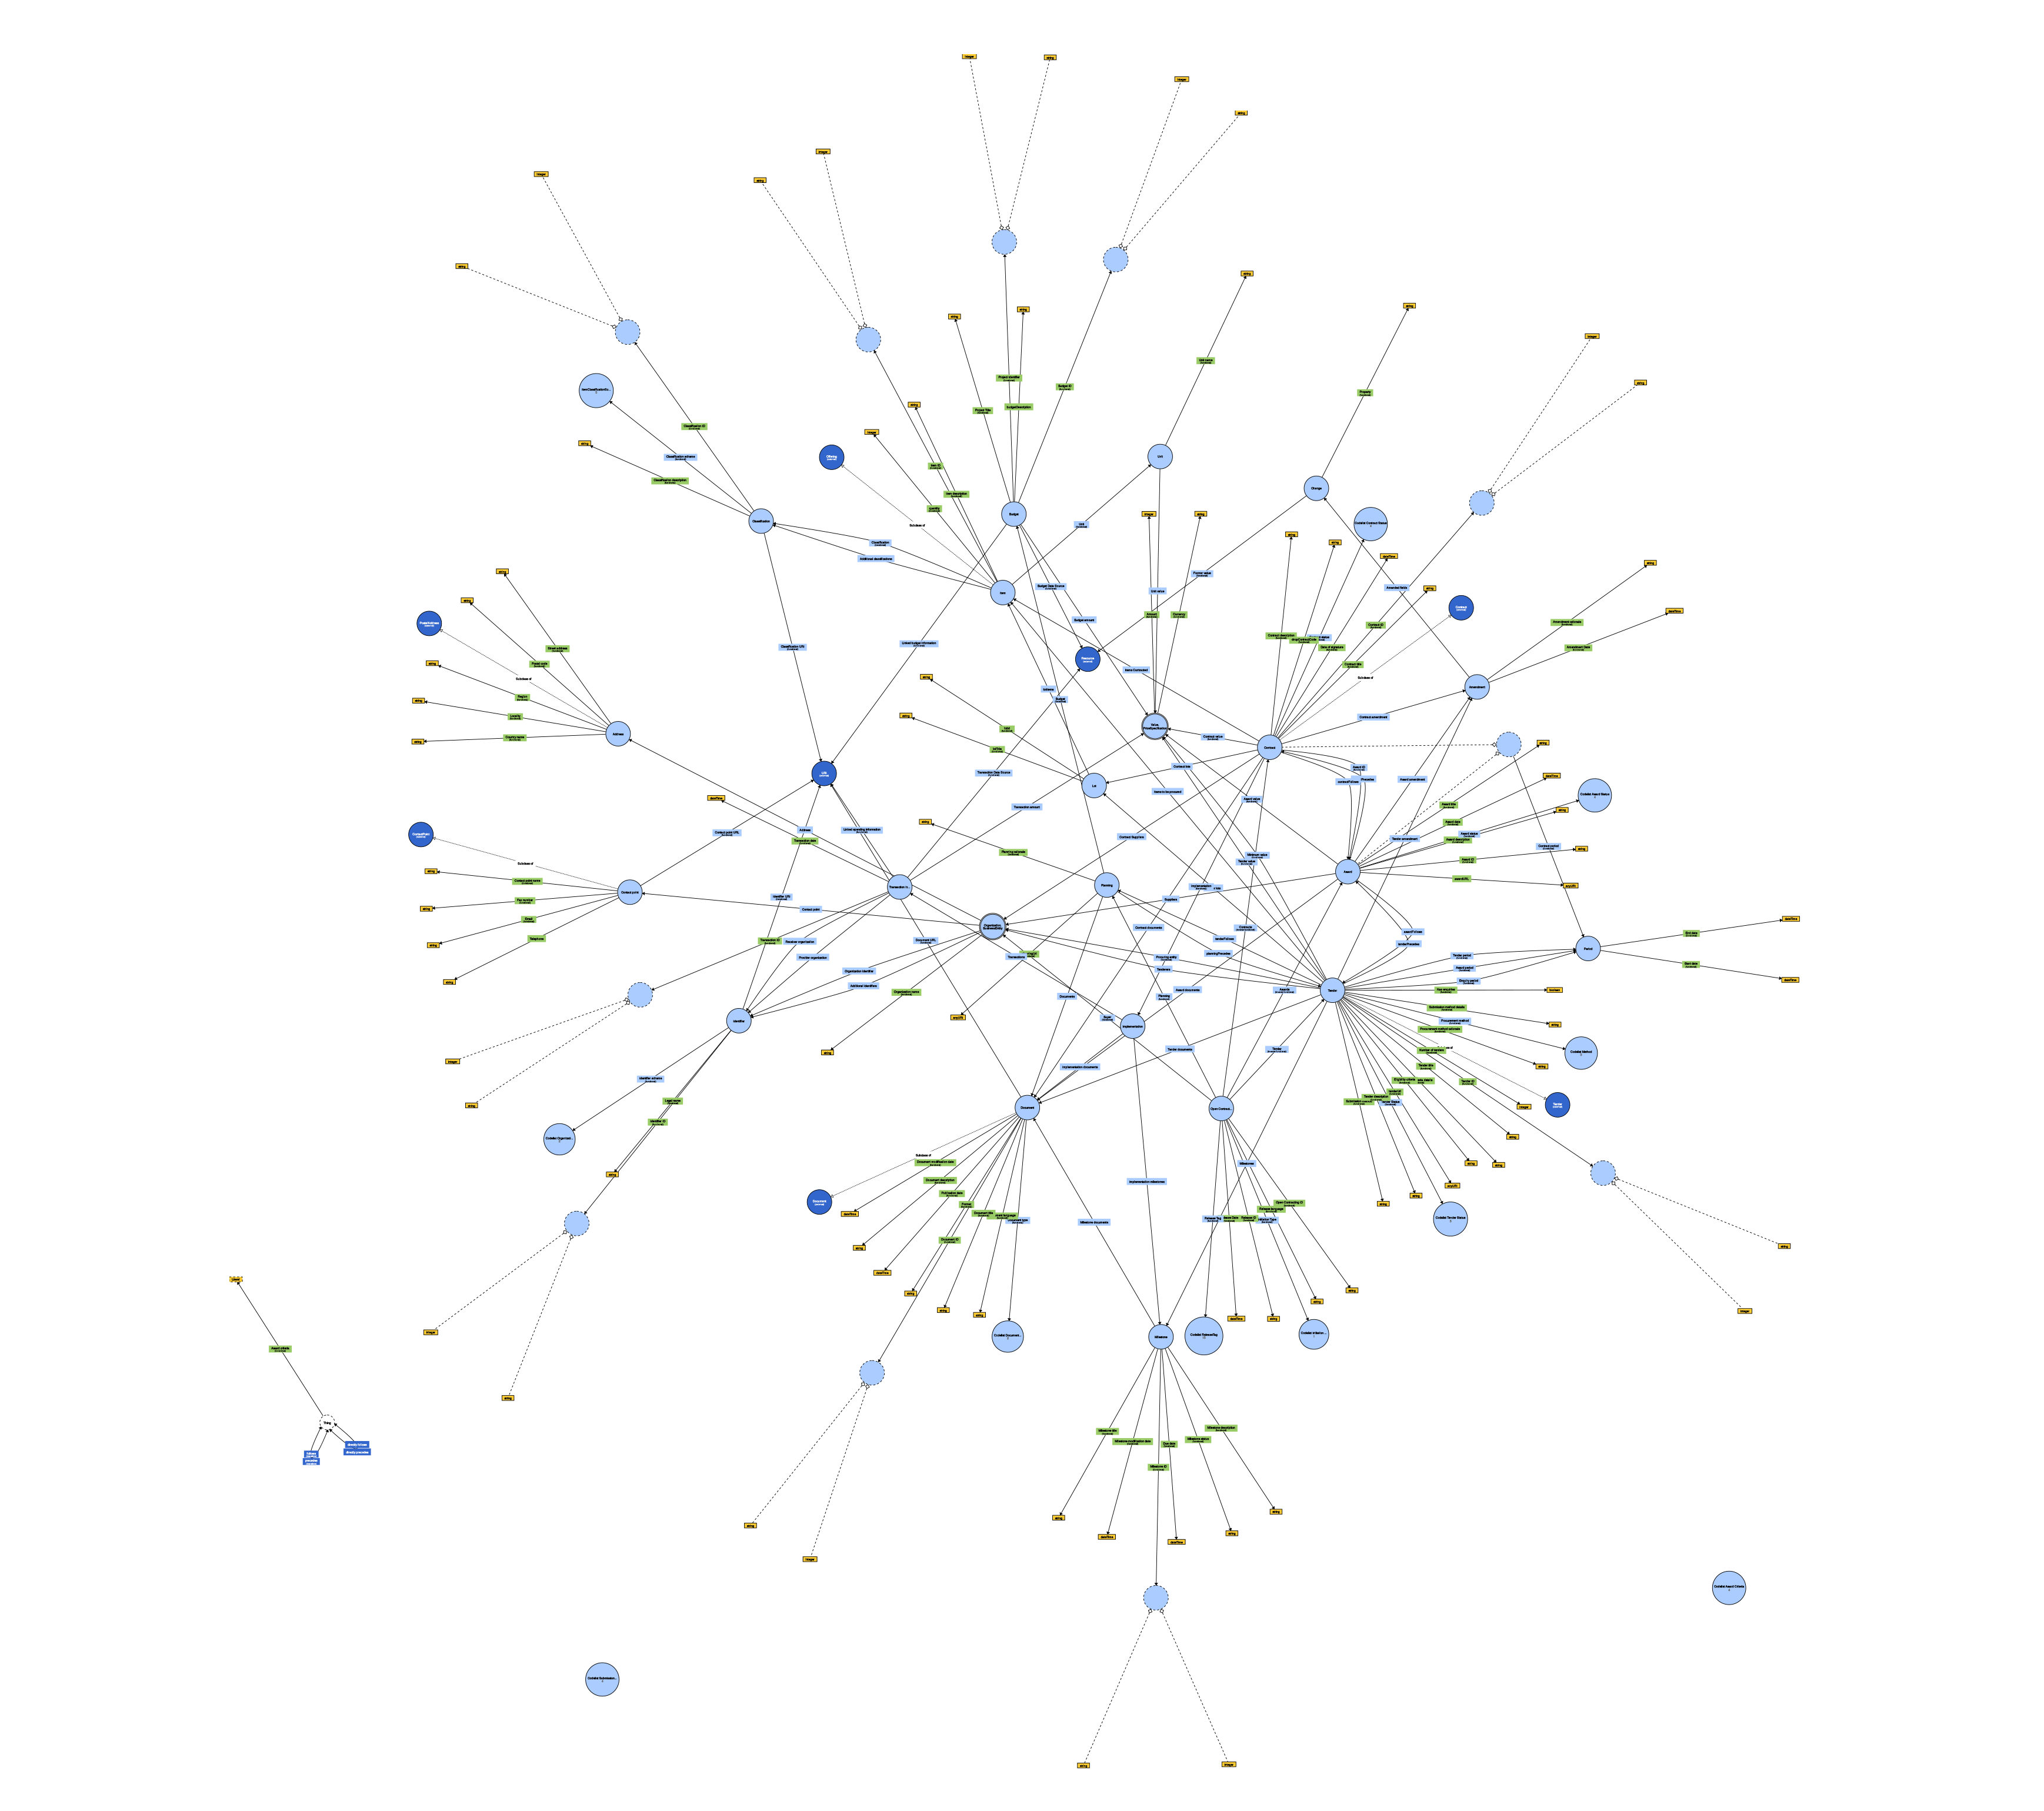
\includegraphics[width=180mm]{figuras/grafoOCDS.png}
    \caption{Grafo de la ontología desarrollada}
    \label{img:grafo ontologia desarrolla}
    \end{figure}

    \begin{figure}[ht!]
        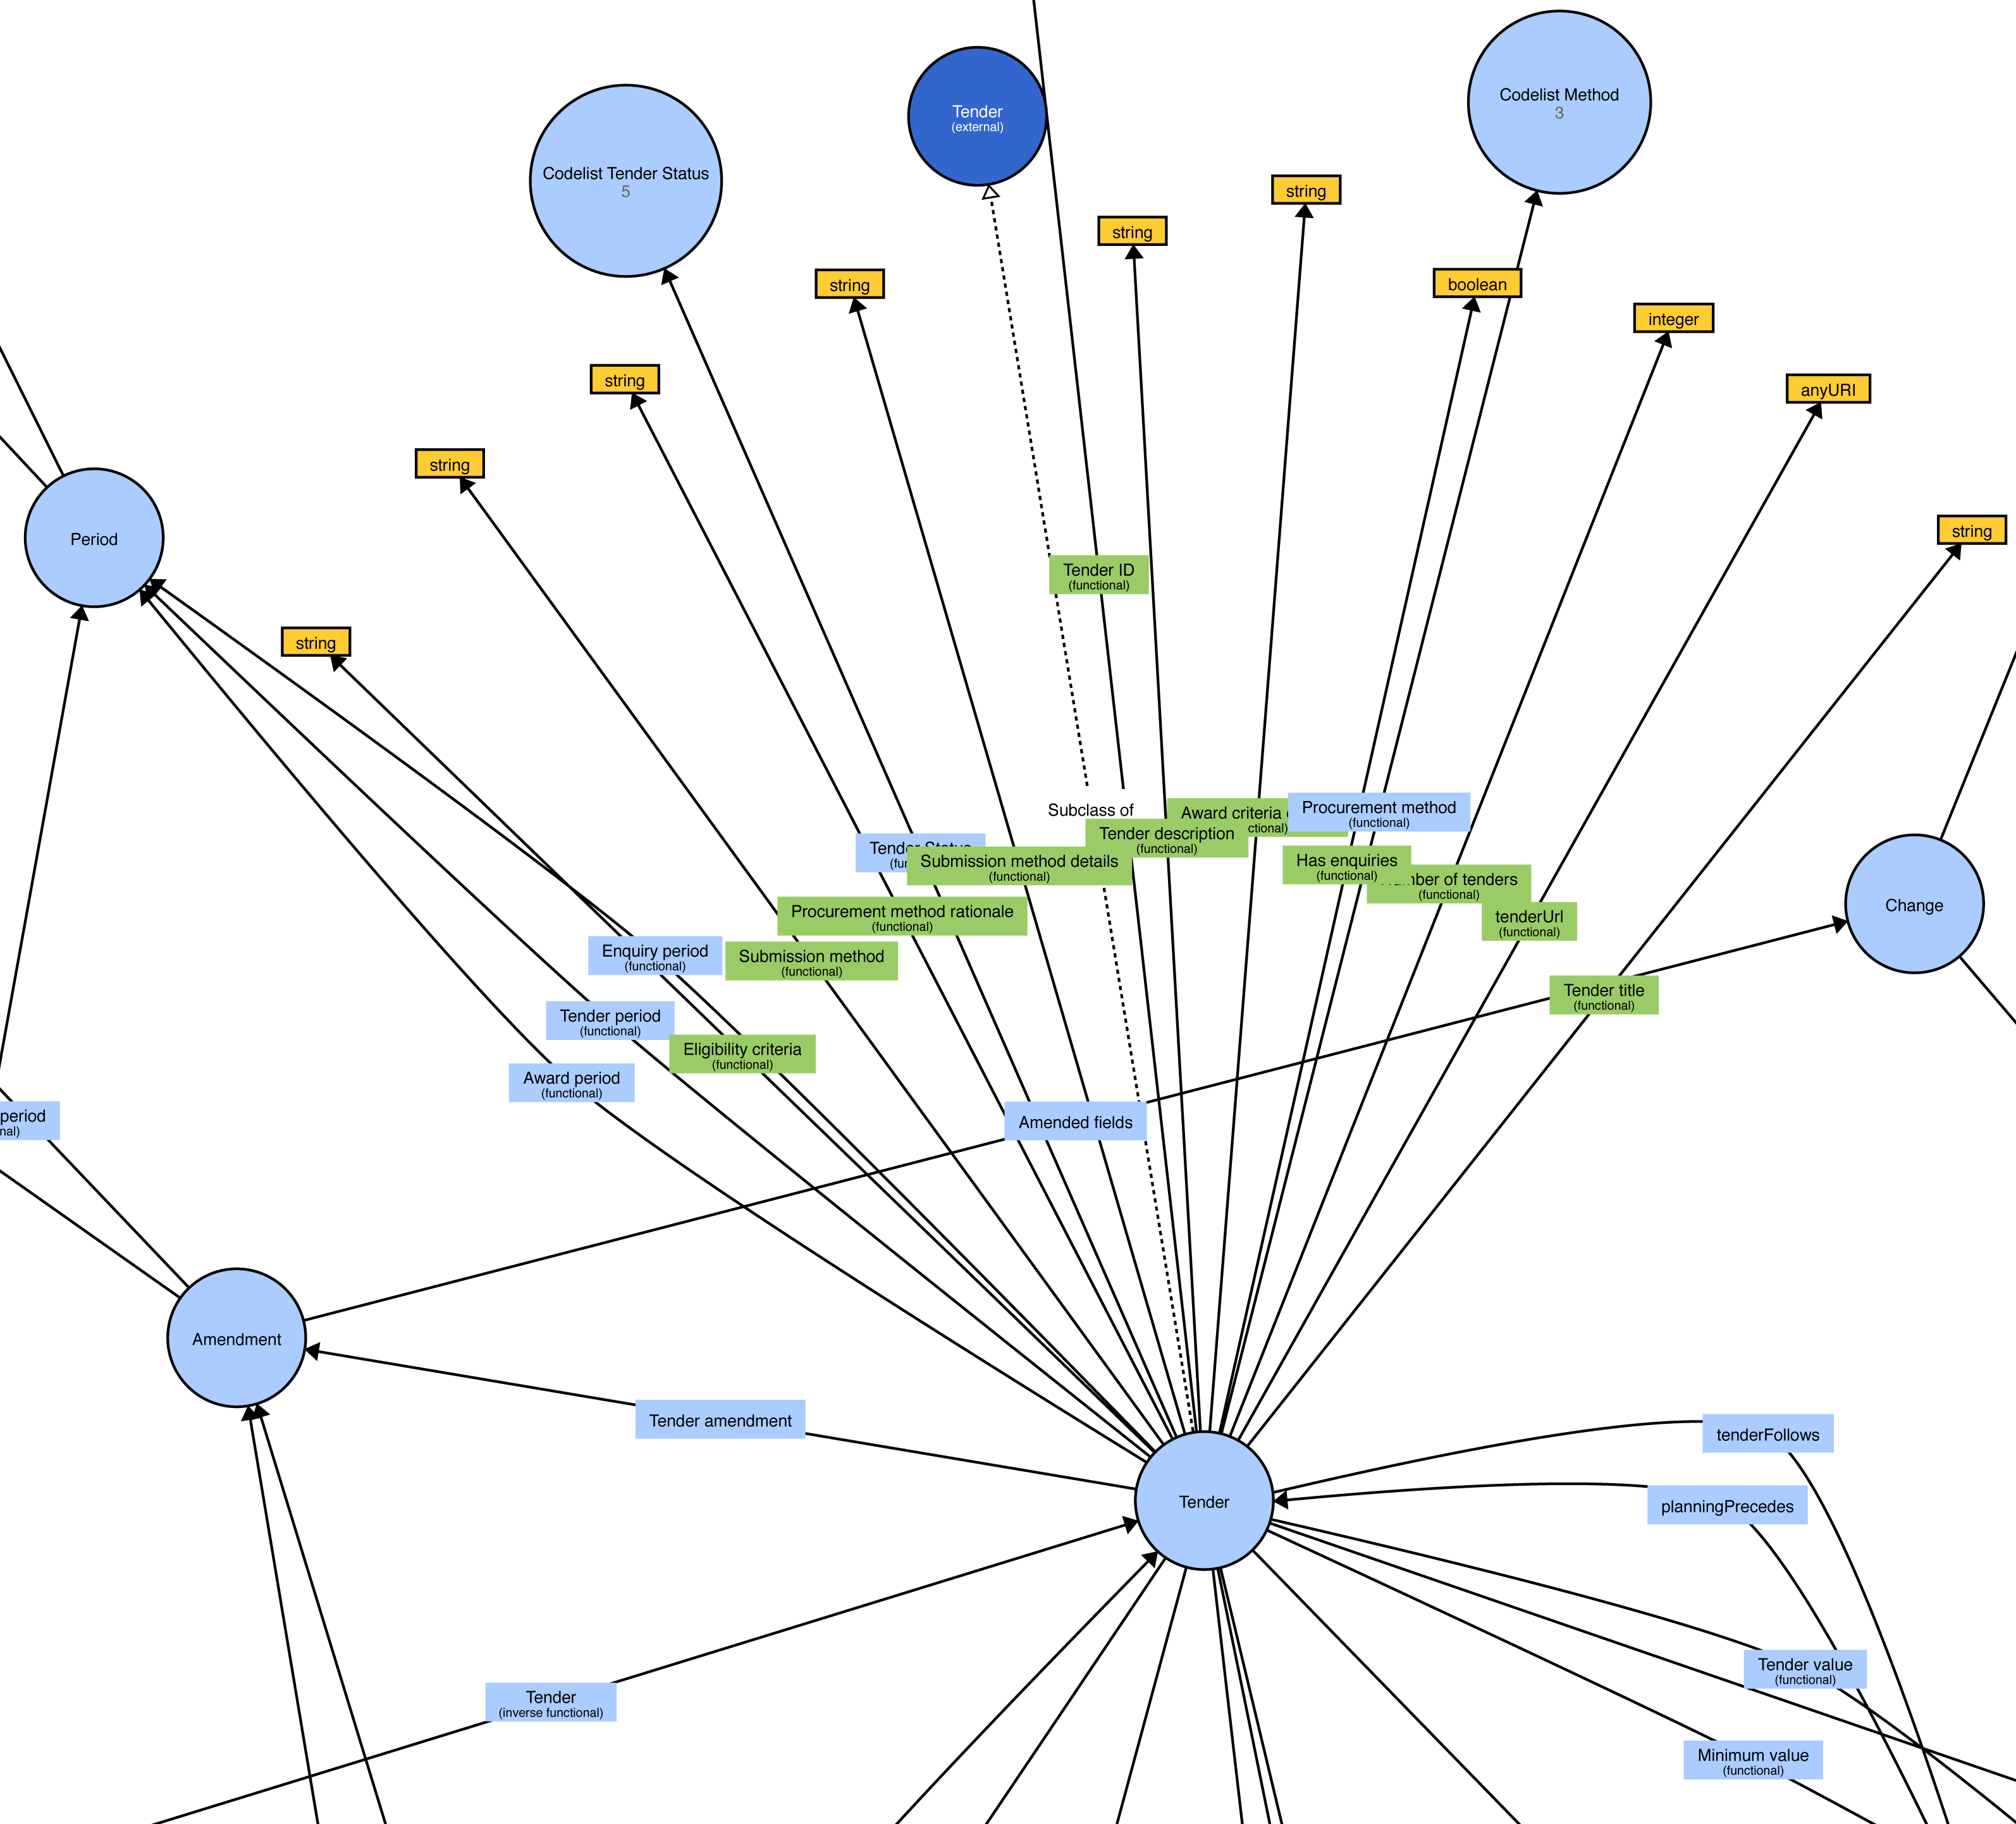
\includegraphics[width=150mm]{figuras/zoomTender.png}
        \caption{Acercamiento del Grafo de la ontología desarrollada en Convocatoria.}
        \label{img:zoomTender}
        \end{figure}


        \begin{figure}[ht!]
            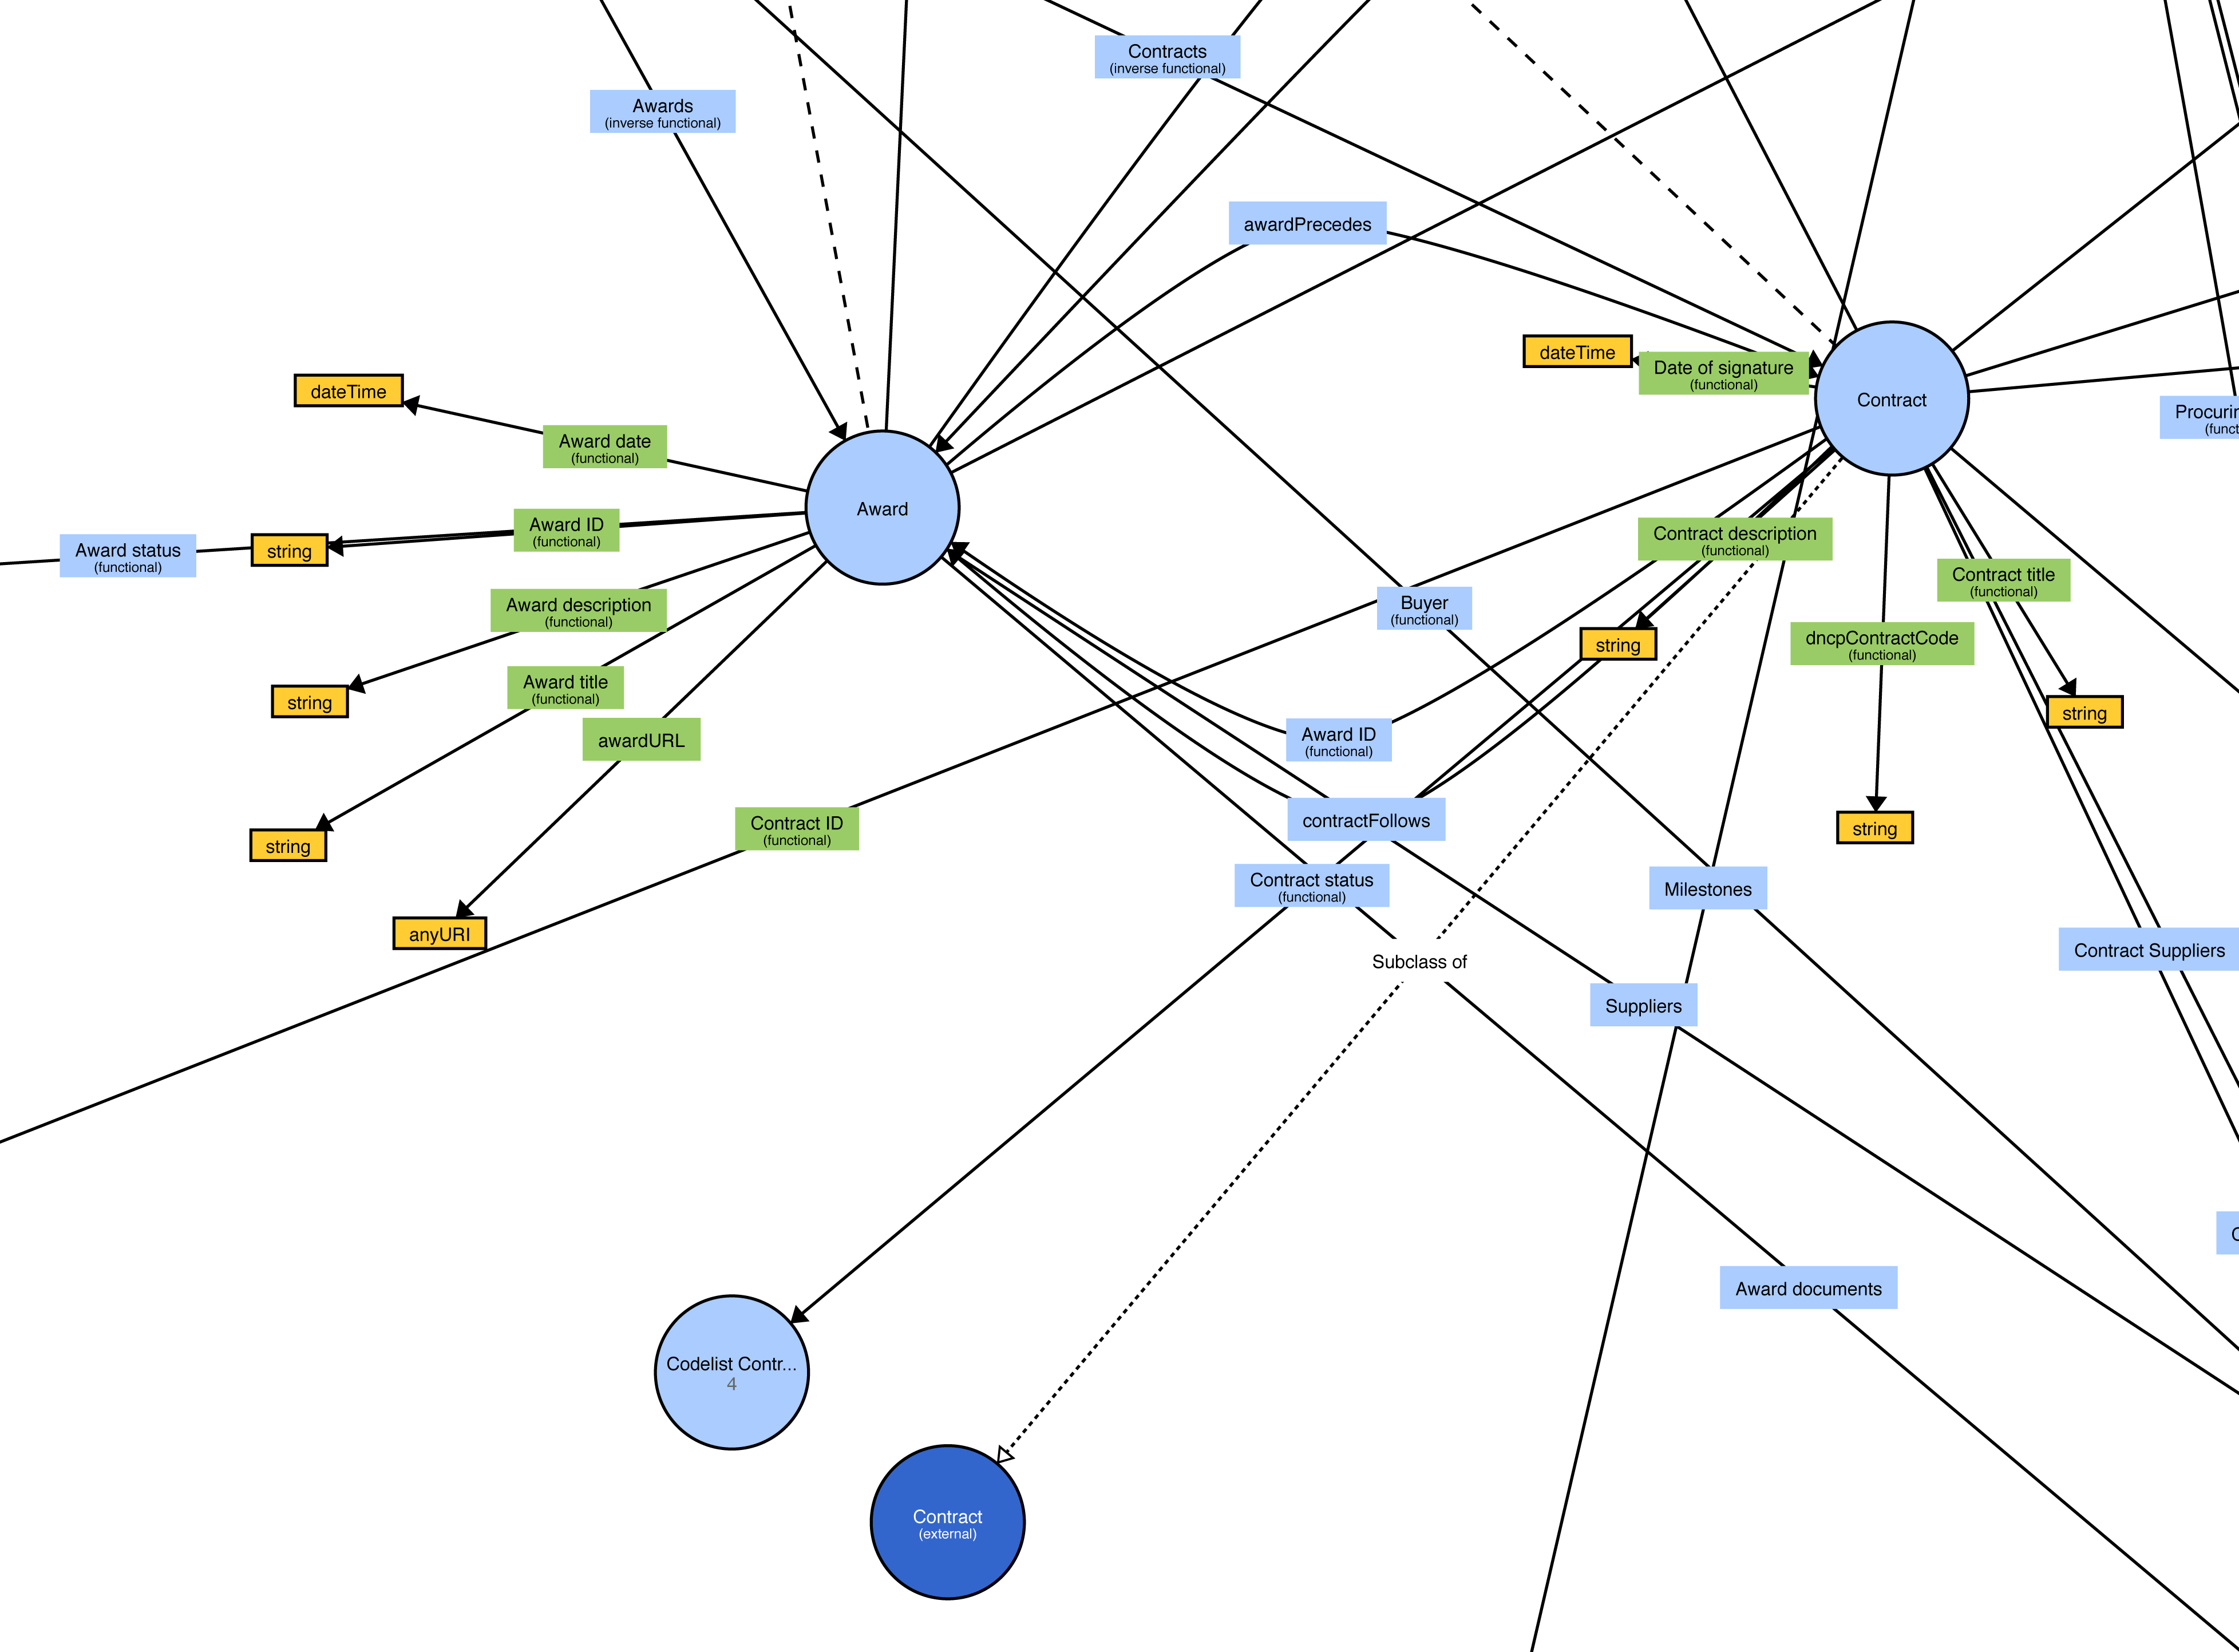
\includegraphics[width=150mm]{figuras/zoomContract.png}
            \caption{Acercamiento del Grafo de la ontología desarrollada en Contracto.}
            \label{img:zoomContract}
            \end{figure}



\section{Discusión del Capitulo}

En este capítulo se desarrolló una ontología teniendo como base de conocimiento un recurso no-ontológico (OCDS). Se utilizó la metodología NeOn y el software Protégé para el desarrollo de ontología. Las actividades principales fueron la planificación de actividades, especificación de los requerimientos, el reuso de recursos ontológicos y no-ontológicos. El resultado de todo este proceso fue una ontología desarrollada en lenguaje OWL que responde a la base de conocimiento de la OCDS y al esquema de datos de la DNCP teniendo en cuenta las buenas prácticas de desarrollo de ontologías propuestas por la metodología.




